\documentclass[conference]{IEEEtran}
\IEEEoverridecommandlockouts
\usepackage{cite}
\usepackage{amsmath,amssymb,amsfonts}
\usepackage{algorithmic}
\usepackage{graphicx}
\usepackage{textcomp}
\usepackage{xcolor}
\usepackage{booktabs}
\usepackage{multirow}
\usepackage{array}
\usepackage{colortbl}
\usepackage{tikz}
\usetikzlibrary{arrows.meta,calc,positioning,fit,backgrounds}
\usepackage{url}
% Balances the two columns on the last page. Degrades safely if not installed.
\IfFileExists{balance.sty}{\usepackage{balance}}{\providecommand{\balance}{}}
% Clickable citations, references and figure/table links. Must be loaded last.
\usepackage[hidelinks,breaklinks=true]{hyperref}
\hypersetup{
  pdftitle={TriLens-MoE-Stack: A Multi-View Hybrid Framework for Lineage-Aware
            Multi-Drug Antibiotic Resistance Prediction in Escherichia coli
            Using Genomic Data},
  pdfauthor={Faiaz Abrar Zaman Pronoy; Pranto Roy; Sinthia Khandoker;
             Shantanu Barua; Md. Jahirul Islam Zishan; Md. Saiful Bari Siddiqui;
             Swakkhar Shatabda; Md. Golam Rabiul Alam}}

% Figures come from the thesis build. Change this if you move them.
\graphicspath{{figures/}{../../thesis/images/}}

% Long drug names break IEEE's narrow columns unless we allow these breaks.
\hyphenation{tri-me-tho-prim-sul-fa-me-tho-xa-zole amo-xi-cil-lin-cla-vu-la-nate
cip-ro-flo-xa-cin cef-ta-zi-di-me ce-fo-ta-xime gen-ta-mi-cin am-pi-cil-lin
be-ta-lac-ta-mase pan-ge-nome phy-lo-group ge-no-mic re-sis-tance
mixture-of-ex-perts}

% ---- helper used by the architecture figure (copied from the thesis preamble) ----
\definecolor{cin}{RGB}{150,190,230}
\definecolor{cexp}{RGB}{150,205,170}
\definecolor{cgate}{RGB}{242,205,120}
\definecolor{cmeta}{RGB}{234,150,150}
\definecolor{cout}{RGB}{200,165,225}
\definecolor{blueedge}{RGB}{46,104,178}
\definecolor{bluefill}{RGB}{222,235,250}
\definecolor{greenedge}{RGB}{61,129,86}
\definecolor{greenfill}{RGB}{220,242,225}
\definecolor{rededge}{RGB}{207,68,59}
\definecolor{redfill}{RGB}{255,219,215}
\definecolor{headgrey}{RGB}{232,236,241}
\definecolor{oursblue}{RGB}{222,235,250}
\newcommand{\blk}[6]{%
 \pgfmathsetmacro{\ox}{0.30*#5}\pgfmathsetmacro{\oy}{0.30*#5}
 \fill[#6,fill opacity=0.45] (#1,#2-#4/2) rectangle (#1+#3,#2+#4/2);
 \fill[#6!60!black,fill opacity=0.45] (#1,#2+#4/2)--(#1+\ox,#2+#4/2+\oy)--(#1+#3+\ox,#2+#4/2+\oy)--(#1+#3,#2+#4/2)--cycle;
 \fill[#6!80!black,fill opacity=0.45] (#1+#3,#2+#4/2)--(#1+#3+\ox,#2+#4/2+\oy)--(#1+#3+\ox,#2-#4/2+\oy)--(#1+#3,#2-#4/2)--cycle;
 \draw[line width=0.32mm] (#1,#2-#4/2) rectangle (#1+#3,#2+#4/2);
 \draw[line width=0.32mm] (#1,#2+#4/2)--(#1+\ox,#2+#4/2+\oy)--(#1+#3+\ox,#2+#4/2+\oy)--(#1+#3,#2+#4/2);
 \draw[line width=0.32mm] (#1+#3+\ox,#2+#4/2+\oy)--(#1+#3+\ox,#2-#4/2+\oy)--(#1+#3,#2-#4/2);}

\begin{document}

\title{TriLens-MoE-Stack: A Multi-View Hybrid Framework for\\
Lineage-Aware Multi-Drug Antibiotic Resistance Prediction\\
in \textit{Escherichia coli} Using Genomic Data}

% All authors share one affiliation, so we use a single centred author block.
% Eight side-by-side \IEEEauthorblock columns would overflow the page width.
\author{%
\IEEEauthorblockN{Faiaz Abrar Zaman Pronoy, \;
Pranto Roy, \;
Sinthia Khandoker, \;
Shantanu Barua,\\
Md. Jahirul Islam Zishan, \;
Md. Saiful Bari Siddiqui, \;
Swakkhar Shatabda, \;
Md. Golam Rabiul Alam\textsuperscript{*}}
\IEEEauthorblockA{\textit{Department of Computer Science and Engineering, BRAC University}\\
}
}

\maketitle

\begin{abstract}
Machine learning can predict antibiotic resistance from a bacterial genome far
faster than a laboratory test, and reported accuracy is often very high. We ask
what that accuracy measures. Because bacteria reproduce clonally, a collection of
strains is a set of near-identical families rather than independent samples, so a
random split lets a model score well by recognising the family instead of the
biology. On 6{,}962 public \textit{Escherichia coli} genomes labelled for seven
antibiotics we built TriLens-MoE-Stack, which reads three genomic views and lets a
mixture-of-experts gate weight them per strain and per drug. Average PR-AUC is
0.849 under a random split and falls to 0.634 under a sequence-type lineage
holdout. We show part of that fall is not model failure: holding out lineages
lowers test prevalence by 2.5 to 12.1 percentage points, and prevalence is exactly
the no-skill baseline of PR-AUC. Resampling the holdout test set to the training
prevalence, without retraining and without discarding any resistant strain,
recovers 0.723, giving an adjusted gap of 0.126 rather than the raw 0.215. The
seven drugs then separate into two groups: three lose 0.017 to 0.031 and four lose
0.176 to 0.244, with nothing between. Meanwhile the mean very major error rate
rises from 0.249 to 0.559 while the accuracy-style measure barely moves. We
conclude that one random-split score is insufficient evidence in this field, and
that generalisation depends on each drug's resistance mechanism.
\end{abstract}

\begin{IEEEkeywords}
antimicrobial resistance, data leakage, genomic prediction, lineage holdout,
mixture-of-experts, multi-view learning, population structure, prevalence
correction
\end{IEEEkeywords}

% =====================================================================
\section{Introduction}
\label{sec:intro}
% =====================================================================

Antibiotic resistance is a serious health problem. In 2019 an estimated 4.95
million deaths were linked to resistant bacterial infections, and 1.27 million of
those were caused directly by the resistance \cite{murray2022}. Both numbers are
higher than the deaths from HIV/AIDS or malaria in the same year. The trend is not
improving. WHO reports that about one bacterial infection in six no longer responds
to the antibiotic first chosen for it, and that more than 40\% of the
bacteria-antibiotic pairs it tracks became harder to treat between 2018 and 2023
\cite{who2025glass}. A separate forecast projects 39 million deaths between 2025
and 2050 \cite{naghavi2024}.

The problem is also a daily one. A doctor treating an infection needs to know which
antibiotic will work. A laboratory culture test answers this, but it takes 18 to 72
hours \cite{ren2022,who2019}, and the patient cannot wait. So the doctor picks a
drug before the result arrives, often a broad-spectrum one to be safe. That choice
feeds the same resistance problem it is trying to avoid. Reading a genome is much
faster. If a model can predict resistance from the genome, the answer comes in
minutes. Many groups have tried this, and reported accuracy is often very high
\cite{moradigaravand2018,ren2022,wang2025}.

\subsection{Why This Problem Is Worth Working On}

Three practical gaps keep this from being solved, and each one shaped our design.

The first is \textbf{time}. Culture takes days, and some bacteria cannot be grown
in a laboratory at all, so for those strains the wait produces no answer.

The second is \textbf{coverage}. Most published tools predict one drug at a time.
But a doctor does not choose between one drug and nothing. The doctor compares
several drugs and picks the best remaining option. So we treat resistance as a
multi-label problem and predict all seven antibiotics in one pass.

The third is \textbf{reach}. Many tools work by looking up known resistance genes
in a database. If a strain is resistant through a gene the database does not list,
the tool returns nothing useful. A learned model can pick up patterns no database
holds, so we learn from the whole genome instead of matching a gene list.

A fourth problem sits behind all three. Most models predict but cannot say why. We
cannot tell whether a model learned a gene that causes resistance or only learned
which family the strain belongs to. From the outside these look the same. Only one
of them is biology.

Working on these problems led us to two deeper issues behind the high scores in the
literature. One is how the genome is turned into features. The other is how the
model is tested.

\subsection{The First Problem: One View Is Not Enough}

Resistance arises in two ways. In the first, the bacterium changes one letter
inside one of its own genes. That changes the shape of the protein the drug
attacks, so the drug stops working. Mutations in \textit{gyrA} and \textit{parC}
cause ciprofloxacin resistance this way. In the second, the bacterium picks up a
whole new gene from another bacterium. The new gene makes an enzyme that destroys
the drug. A TEM-1 beta-lactamase causes ampicillin resistance this way, and the
gene often travels on a plasmid.

One view of the genome cannot catch both. A SNP view cannot see a gene that simply
arrived, because that gene is not a mutation. A gene presence view cannot see one
changed letter, because the gene is present in resistant and susceptible strains
alike. Some studies do use more than one view, but they mix the views with weights
fixed before training. That assumes every view is equally useful for every drug,
and we show later that it is not.

\subsection{The Second Problem: The Test Itself}

Bacteria reproduce by copying themselves. They do not mix genes the way humans do.
So a collection of 6{,}962 strains is not 6{,}962 independent samples. It is a few
hundred families whose members are nearly identical inside each family.

A normal random split cuts every family in half. Some members go to training and
some to testing, so the test set holds strains with near-copies in training. A model
can then score high by learning ``this looks like family 73, and family 73 is
resistant.'' It never has to learn which gene causes resistance. Such a model works
on strains resembling what it has seen and fails on a truly new one, which is
exactly the case where the doctor needs help.

Some studies noticed this and split by population structure \cite{yu2025,hu2024}.
But we found a second effect that nobody has reported. Holding out whole families
also changes how many test strains are resistant, and PR-AUC is read against that
number. So part of the measured drop belongs to the metric, not the model. Nobody
has separated the two.

\subsection{Our Contributions}

This paper makes five contributions.

\begin{enumerate}
\item \textbf{A three-view model with a learned gate.} TriLens-MoE-Stack reads
three genomic views, and a mixture-of-experts gate learns how much to trust each
view for each strain and each drug instead of using fixed weights.

\item \textbf{A prevalence correction for lineage-aware testing.} We measure how
much of the drop comes from the shift in test prevalence and separate it from the
real loss of generalisation. As far as we know this is new for this task.

\item \textbf{Per-antibiotic reporting of the corrected drop.} Reported per drug
instead of as one average, the drop splits into two groups with an empty space
between them. A single average hides this.

\item \textbf{A fix for a problem in gated attention.} Standard gated attention
breaks down on binary gene data. We correct it, and the ablation shows the fix is
visible only under the lineage holdout, which supports our main argument.

\item \textbf{Honest reporting of negative results.} Attention did not explain the
model, the neural part adds almost nothing on unfamiliar lineages, and no
antibiotic met the clinical error limits. We report all three.
\end{enumerate}

Together these answer five questions. RQ1: can a hybrid of neural lenses and
classical learners predict resistance from genomic data? RQ2: how much does each
part contribute? RQ3: can attention and gate weights say which genes drive a
prediction? RQ4: how much of the score is resistance mechanism and how much is
population structure? RQ5: does the model still work on an unseen family?

Section~\ref{sec:lit} reviews earlier work, Section~\ref{sec:method} describes the
data and the model, Section~\ref{sec:results} gives the results, and
Sections~\ref{sec:discussion} and \ref{sec:conclusion} discuss and conclude.

% =====================================================================
\section{Literature Review}
\label{sec:lit}
% =====================================================================

\subsection{Background Terms}

We use the standard three-letter codes for the seven antibiotics throughout: AMP
for ampicillin, CIP for ciprofloxacin, AMC for amoxicillin-clavulanate, SXT for
trimethoprim-sulfamethoxazole, GEN for gentamicin, CTX for cefotaxime and CAZ for
ceftazidime.

Two terms carry weight later and are worth fixing now. A \textit{pan-genome} is the
union of all genes seen anywhere in a collection, rather than the genes of one
chosen reference strain. A gene that only some strains carry does not exist in a
single-reference view at all, and acquired resistance genes are exactly that kind of
gene. A \textit{sequence type} (ST) is a family label from multi-locus sequence
typing, so strains sharing an ST are close relatives, whereas a \textit{phylogroup}
is a far broader grouping and \textit{E. coli} has only eight. The gap between those
two levels of resolution turns out to decide our main result.

\subsection{How Other Studies Represent the Genome}

Some studies use the pan-genome and gene presence. Moradigaravand et al.
\cite{moradigaravand2018} worked on 1{,}936 \textit{E. coli} strains with gradient
boosting and random forest. Their feature importance recovered \textit{gyrA} and
\textit{parC}, which is a good sign that the model found real biology. Her and Wu
\cite{her2018} scored gene clusters with a genetic algorithm, but their collection
had only 59 strains.

Other studies work at nucleotide level. Serajian et al. \cite{serajian2024} used
31-mers on \textit{M. tuberculosis}. Gao et al. \cite{gao2024} applied $k$-mers to \textit{A. baumannii} and found a
categorical agreement greater than 95\%. The use of unitigs done on \textit{P.
aeruginosa} by Do et al. \cite{do2024} resulted in a decrease of the AUC which was
above 0.929 in training and approximately 0.77 in an independent collection. That drop is
close to what we also observe, although they did not analyse why it happened.

A few studies combine two or more views. Ren et al. \cite{ren2022} used one-hot
and FCGR encodings of whole-genome sequences on Giessen and public \textit{E. coli}
data, and reported AUC around 0.96 with random forest. Wang et al.
\cite{wang2025} used SNPs together with gene presence on \textit{H. pylori} and
used SHAP for interpretation. Siddiqui and Tarannum \cite{siddiqui2025} combined
SNP motifs with the pan-genome on 809 Giessen \textit{E. coli}.

Across all of these, classical tree models are hard to beat. The same pattern is
reported for tabular data in general \cite{grinsztajn2022,shwartzziv2022}. Even
TabNet \cite{arik2021}, which was designed for tabular data, does not always beat
a well-tuned gradient boosting model. We test this ourselves in
Section~\ref{sec:results}.

\subsection{How Other Studies Combine Views and Models}

Since no single view captures both mechanisms, the natural next step is to use more
than one. Studies that do this almost always join the views by concatenation, or
average the outputs of separate models with weights fixed before training. Both
carry the same hidden assumption: that every view deserves equal trust for every
drug. That assumption is testable, and for our data it is wrong. This is why we use
a mixture-of-experts gate, and why Section~\ref{sec:results} reports what the gate
actually learned rather than only that it helped.

On the model side, stacked generalisation \cite{wolpert1992} is the standard way to
combine learners that fail differently. It is well established elsewhere but rarely
used here, where most papers report a single model family.

\subsection{Practical Barriers Reported by Others}

Two barriers come up repeatedly and shaped our design. First, a model trained on
one collection often cannot be run on another at all, because the two use different
reference genomes and therefore different feature spaces. Do et al. \cite{do2024}
report the size of the drop when a model does move across collections, and Nsubuga
et al. \cite{nsubuga2024} train on \textit{E. coli} from England and test on an
independent collection from Uganda, Nigeria and Tanzania. Their result matches ours
in kind: a model that looks strong at home loses a great deal on strains from
somewhere it has not seen. Second, resistant strains are the rare class for most
drugs, so accuracy stays high while the rare class is missed, yet several studies
report accuracy anyway. Section~\ref{sec:method} addresses both.

\subsection{How Other Studies Test Their Models}

Clonal population structure is well known in bacterial genome-wide association
studies, where the correction is built into the model rather than added later.
Saber and Shapiro \cite{saber2020} showed on simulated data that population
structure makes a causal variant hard to separate from a linked one. Lees et al.
\cite{lees2020} fit a regression across the whole pan-genome so variants compete
inside one model.

The prediction side of the field has mostly not adopted this, and there is a reason.
An association study asks which variant causes the trait, so family background is a
threat and must be removed. A prediction study only asks how well the trait can be
guessed, and family background is a fair source of signal there. The problem appears
only when the model meets an unseen family, and a random split never creates that
situation.

We reviewed sixteen studies. Fourteen of them predict a resistance phenotype. The
other two are a review \cite{yun2024} and a gene classification tool
\cite{arangoargoty2018}, so we do not count them here.

Of those fourteen, \textbf{four} engage with population structure in some way. Two
make it the main design. Yu et al. \cite{yu2025} used phylogeny-aware splits over
more than 24{,}000 genomes and five pathogens, and found that scores drop when
structure is ignored. Hu et al. \cite{hu2024} compared random, phylogeny-aware and
homology-aware folds across 78 pathogen-antibiotic pairs, and found that scores
fall clearly under phylogeny-aware folds.

The other two report it as a secondary check. Moradigaravand et al.
\cite{moradigaravand2018} held out the ST131 family in a supplementary analysis and
reported that accuracy fell by about 0.28 against a random test set of the same
size. Orcales et al. \cite{orcales2024} provide MLST-blocked cross-validation as an
option.

So we do not claim that lineage-aware splitting is new. It is not, and we cite the
four studies that engage with it. Our claim is smaller than that. \textbf{None of
those four corrects the metric for the prevalence shift that such a split causes,
and none reports the resulting drop for each antibiotic separately.} Those two gaps
are what this paper works on.

Table~\ref{tab:related} places our work next to the six closest studies. We chose
these six because they work on the same organism, the same collections, or the
same question about population structure.

\begin{table*}[t]
\caption{Our work compared with the six closest studies. ``N/R'' means the study
does not report that property. It does not mean the study attempted it and failed.}
\label{tab:related}
\centering
\small
\setlength{\tabcolsep}{4pt}
\renewcommand{\arraystretch}{1.25}
\begin{tabular}{|>{\raggedright\arraybackslash}p{2.4cm}|>{\raggedright\arraybackslash}p{2.2cm}|>{\raggedright\arraybackslash}p{2.9cm}|>{\raggedright\arraybackslash}p{2.5cm}|>{\centering\arraybackslash}p{1.4cm}|>{\raggedright\arraybackslash}p{1.9cm}|>{\raggedright\arraybackslash}p{1.7cm}|}
\hline
\rowcolor{headgrey}
\textbf{Study} & \textbf{Organism, scale} & \textbf{Genomic views} & \textbf{Evaluation split} & \textbf{Prev. fix} & \textbf{Interpret.} & \textbf{External set} \\ \hline
Moradigaravand et al. \cite{moradigaravand2018} & \textit{E. coli}, 1{,}936 strains, 11 drugs & Pan-genome, structure as a feature & Random; ST131 holdout in a supplement & N/R & Feature importance (\textit{gyrA}, \textit{parC}) & N/R \\ \hline
Ren et al. \cite{ren2022} & \textit{E. coli}, 987 + 1{,}509 strains, 4 drugs & One-hot and FCGR encodings & Stratified cross-validation & N/R & Associated mutations reported & Trained on one, tested on another \\ \hline
Orcales et al. \cite{orcales2024} & \textit{E. coli}, 1{,}936 strains & Single view & Cross-validation; MLST-blocked option & N/R & N/R & N/R \\ \hline
Wang et al. \cite{wang2025} & \textit{H. pylori}, 296 strains, 4 drugs + MDR & SNPs and gene presence & Random & N/R & SHAP & None reported \\ \hline
Siddiqui and Tarannum \cite{siddiqui2025} & \textit{E. coli} (Giessen), 809 strains, 4 drugs & SNP motifs and pan-genome & Stratified 80/20 & N/R & Attribution & N/R \\ \hline
Yu et al. \cite{yu2025} & 5 pathogens, over 24{,}000 strains & Single view & Phylogeny-aware & N/R & N/R & N/R \\ \hline
\rowcolor{oursblue}
\textbf{This work} & \textbf{\textit{E. coli}, 6{,}962 strains, 7 drugs} & \textbf{SNP blocks, gene presence, gene statistics, gated} & \textbf{Random and MLST lineage holdout} & \textbf{Yes} & \textbf{SHAP and attention} & \textbf{Giessen, retrained} \\ \hline
\end{tabular}
\renewcommand{\arraystretch}{1.0}
\end{table*}

If we look only at the scale and views columns, our work is not very different
from the others. Our collection is larger than most single-organism studies but
smaller than the multi-pathogen one. Using several views is a smaller difference
than it sounds, because Ren et al. and Siddiqui and Tarannum also combine views.
So we do not claim that our model is new just because it reads three inputs.

The difference is in the last three columns. Four of the fourteen studies engage
with population structure, two as their main design and two as a secondary check,
but none of the four corrects for what that split does to the metric. That is the
gap this paper works in.

% =====================================================================
\section{Methodology}
\label{sec:method}
% =====================================================================

\subsection{Dataset}

We use the open \textit{E. coli} dataset published by Arcadia Science
\cite{morin2024,york2025}. It came out in two parts. The first release gives the
variant calls against a pan-genome reference, together with the laboratory result
table and the strain information. The second release gives gene presence and
absence for all strains as PLINK files. Our SNP views come from the first release
and our gene presence view comes from the second.

We chose it for three reasons. The variant calls were already quality checked by
the publishers, which removes a large source of difference between studies. It uses
a pan-genome rather than a single reference, so genes that only some strains carry
are included. And another group has published their own analysis of the same
strains, so we can compare findings later.

Three files had to match before we could use a strain: the variant file is listed by
sequencing accession, the result file by genome name, and a separate mapping file
joins them. We kept a strain only if it appeared in all three, leaving
\textbf{6{,}962} strains. Every experiment here uses these strains. The three files
disagree on how many strains exist (6{,}985, 6{,}983 and 7{,}043 respectively). We
did not force them to agree; we kept the strains present wherever we needed them.

\subsection{Labels and Missing Values}

Each laboratory result is resistant, intermediate or susceptible, and blank when no
test was done. Resistant and intermediate were coded as 1 and susceptible was coded
as 0. We have included intermediate with resistant because: the publishers have done
the same and so our labels will be comparable, and clinically an intermediate outcome
implies that normal dose will not be strong enough, and so it is safer to label it as
resistant. There is one side effect. In our results, the categorical agreement is the
same as plain accuracy since no intermediate category remains.

Not all of the strains were evaluated for sensitivity to all of the drugs. Rather than
discarding incomplete rows, or making guesses, we had a true/false mask of size
$6{,}962 \times 7$ indicating which entries are real. Those entries are solely
considered for training loss and for every metric. \textbf{In this work, no missing
value has been filled anywhere.}

What was left is shown in Table~\ref{tab:labels} and later two columns matter. There
is approximately twice the coverage, 86.7\% in CIP and GEN to 49.1\% in SXT; a
smaller number of labelled strains gives a broader confidence interval. Prevalence
varies about fourfold, from 0.501 for AMP down to 0.118 for GEN. That matters because the
no-skill value of PR-AUC is the prevalence itself, so 0.70 on GEN is a much bigger
gain over chance than 0.70 on AMP.

\begin{table}[t]
\caption{The seven antibiotic labels after cleaning. Coverage is the share of the
6{,}962 strains tested against that drug. Prevalence is the share of those tested
that came back resistant.}
\label{tab:labels}
\centering
\small
\setlength{\tabcolsep}{4pt}
\renewcommand{\arraystretch}{1.15}
\begin{tabular}{|l|r|r|r|r|r|}
\hline
\rowcolor{headgrey}
\textbf{Drug} & \textbf{Res.} & \textbf{Susc.} & \textbf{Tested} & \textbf{Coverage} & \textbf{Prev.} \\ \hline
AMP & 2{,}439 & 2{,}429 & 4{,}868 & 69.9\% & 0.501 \\ \hline
CIP & 1{,}377 & 4{,}656 & 6{,}033 & 86.7\% & 0.228 \\ \hline
AMC & 1{,}180 & 2{,}598 & 3{,}778 & 54.3\% & 0.312 \\ \hline
SXT & 1{,}060 & 2{,}358 & 3{,}418 & 49.1\% & 0.310 \\ \hline
GEN & 710 & 5{,}327 & 6{,}037 & 86.7\% & 0.118 \\ \hline
CTX & 823 & 4{,}586 & 5{,}409 & 77.7\% & 0.152 \\ \hline
CAZ & 780 & 5{,}193 & 5{,}973 & 85.8\% & 0.131 \\ \hline
\end{tabular}
\renewcommand{\arraystretch}{1.0}
\end{table}

\subsection{From Raw Variants to Features}

The variant file is about 1.1 GB compressed. We streamed it once and kept a variant
only if it was a single-nucleotide change (so indels were dropped) and had a minor
allele frequency of at least one per cent. Table~\ref{tab:variants} shows the
result: 535{,}439 kept out of 2{,}451{,}184, or 21.8\%.

\begin{table}[t]
\caption{Variant filtering while building the SNP matrix.}
\label{tab:variants}
\centering
\small
\setlength{\tabcolsep}{4pt}
\renewcommand{\arraystretch}{1.15}
\begin{tabular}{|l|r|}
\hline
\rowcolor{headgrey}
\textbf{Stage} & \textbf{Variants} \\ \hline
Streamed from the variant file & 2{,}451{,}184 \\ \hline
Removed: insertion or deletion & 43{,}799 \\ \hline
Removed: minor allele frequency below 1\% & 1{,}871{,}946 \\ \hline
\rowcolor{oursblue}
\textbf{Kept} & \textbf{535{,}439} \\ \hline
\end{tabular}
\renewcommand{\arraystretch}{1.0}
\end{table}

The frequency filter alone removed 76\% of the variants, most of them present in
only two or three strains. A pattern seen that rarely cannot be expected to hold on
a new strain, so dropping them cost almost nothing.

Genotypes are stored as small whole numbers: zero is the reference allele and 1, 2
or 3 are alternates. We pass these through as numbers rather than one-hot columns.
In our data 83.3\% of calls are reference and 16.3\% are first alternate, while
second and third alternates together are only 2.5\% of non-reference calls, so extra
columns were not worth the memory. Missing genotypes were set to the reference
allele, following the publishers. This is not a harmless choice. Sequencing coverage
is usually lower on plasmids, which is where many resistance genes sit, and that is
part of why GEN is our hardest drug.

\subsection{Reducing the Feature Space}

There are 535{,}439 features for 6{,}962 strains, about 77 candidate features per
sample, so cutting down was necessary rather than optional. We cut at the gene level
because our model reads genes, using two filters.

The first keeps a gene only if it has at least five SNPs across the collection.
Below that we cannot look for a pattern inside the gene, which is the whole point of
our first view. This takes 18{,}975 genes down to \textbf{13{,}799}.

The second ranks genes by importance. For each antibiotic we run a chi-squared test
and keep the top 50{,}000 SNPs for that drug, then train one gradient boosting model
per antibiotic on that smaller set and record how much each gene reduced the error.
Summing this gain across the seven models, we keep the \textbf{5{,}000} genes with
the highest total. Those genes hold 262{,}225 SNPs, about 49\% of what we started
with.

Both filters are fitted on the training part only, and refitted from scratch inside
every split. This is easy to miss and it matters. Choosing features needs the labels,
so if test labels are visible while ranking, the test set decides which features
exist at all and every later score is too high by an unmeasurable amount.

Refitting per split gave one result we did not expect. The gene set chosen under the
lineage holdout shares less than half its genes with the random-split set. So the
resistance signal does not sit in a few genes. It is spread across many genes that
can partly stand in for each other.

\subsection{The Three Genomic Views}

\textbf{View 1: SNP blocks by gene}, shape $6{,}962 \times 5{,}000 \times 64$. For
each strain and kept gene there is a block of 64 slots holding that gene's SNPs,
which catches mutation-type resistance. We set the block length to 64 for a
practical reason. Among the kept genes the smallest has 5 SNPs, the median 32, the
mean 52 and the largest 717. At 64 slots about 28\% of genes are truncated and the
rest are padded with zeros and masked, so a block holds 35 real positions on
average. A shorter block would cut the median gene; a longer one would waste memory
on empty slots.

\textbf{View 2: gene presence and absence}, shape $6{,}962 \times 32{,}441$. This
binary vector says which genes the strain carries and catches acquisition-type
resistance. We deliberately do not filter it to 5{,}000, because a gene that is rare
across the collection can still decide the answer for one strain.

The release stores this matrix as 0 and 2, and nothing states which value means
present, so we tested both readings. If non-zero means present, the median strain
carries about 28{,}700 genes; if zero means present, it carries 3{,}709. An
\textit{E. coli} genome holds about 4{,}000 to 5{,}000 genes, so zero means present.
We report this check because the wrong choice would have raised no error at all. The
model would have trained happily on an inverted matrix and everything after it would
have been silently wrong.

\textbf{View 3: per-gene statistics}, shape $6{,}962 \times 5{,}000 \times 4$. Each
gene is summarised by four numbers from its SNPs: the mean of the alleles, their
variance, the number of positions differing from the reference, and the largest
allele value. This view is rough and cannot locate a mutation inside a gene, but it
is small and stable. The four statistics are standardised to zero mean and unit
variance using the training part only, so no test genome affects the scaling.

\subsection{Model Architecture}

Instead of choosing one view, we include all three and let the model decide which
matters for each drug. Figure~\ref{fig:arch} shows the full design.

\begin{figure*}[t]
\centering
\resizebox{0.92\textwidth}{!}{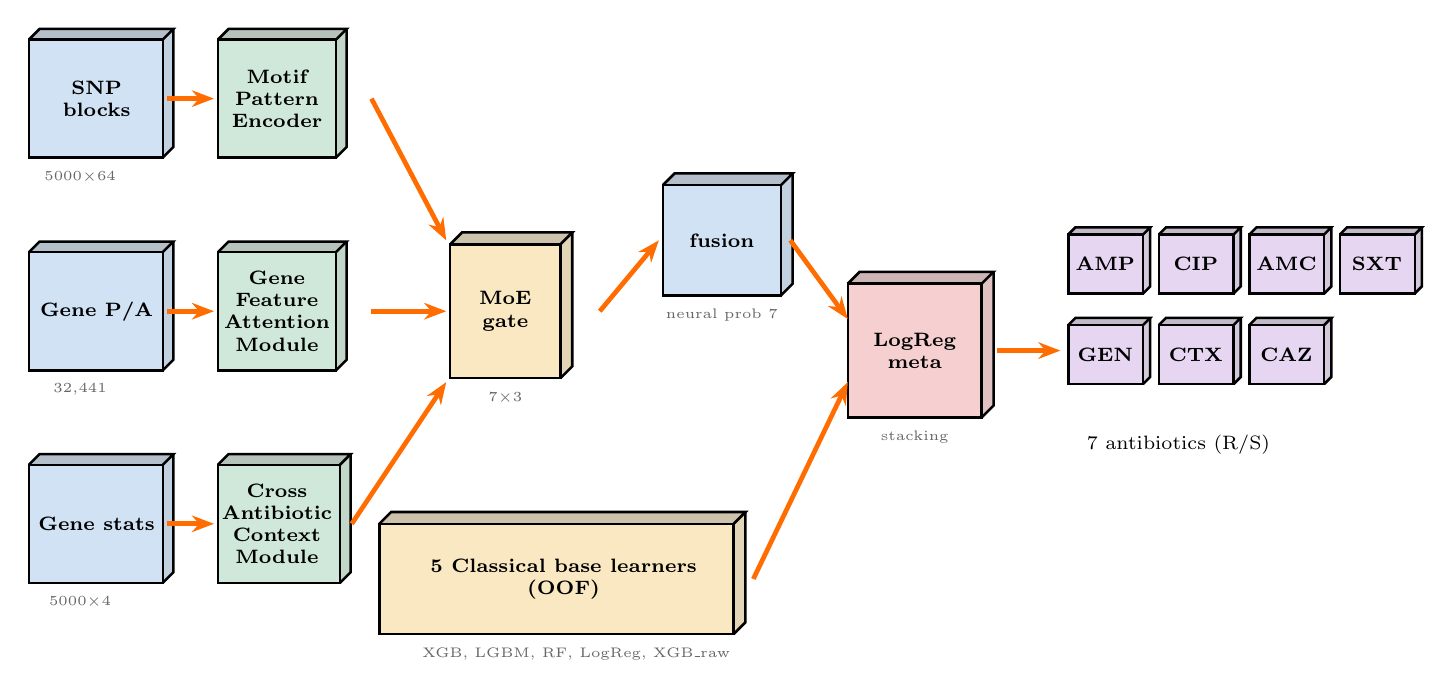
\begin{tikzpicture}[font=\sffamily,>=Stealth,
 ar/.style={-{Stealth[length=2.8mm]},line width=0.6mm,draw=orange!85!red}]
\blk{0}{2.7}{1.7}{1.5}{0.45}{cin}
\node[font=\scriptsize\bfseries,align=center] at (0.86,2.7) {SNP\\blocks};
\node[below,font=\tiny,text=black!60,align=center] at (0.65,1.9) {$5000{\times}64$};
\draw[ar] (1.75,2.7)--(2.35,2.7);
\blk{2.4}{2.7}{1.5}{1.5}{0.45}{cexp}
\node[font=\scriptsize\bfseries,align=center] at (3.15,2.7) {Motif\\Pattern\\Encoder};
\draw[ar] (4.35,2.7)--(5.3,0.9);
\blk{0}{0.0}{1.7}{1.5}{0.45}{cin}
\node[font=\scriptsize\bfseries,align=center] at (0.86,0.0) {Gene P/A};
\node[below,font=\tiny,text=black!60,align=center] at (0.65,-0.8) {$32{,}441$};
\draw[ar] (1.75,0.0)--(2.35,0.0);
\blk{2.4}{0.0}{1.5}{1.5}{0.45}{cexp}
\node[font=\scriptsize\bfseries,align=center] at (3.15,0.0) {Gene\\Feature\\Attention\\Module};
\draw[ar] (4.35,0.0)--(5.3,0);
\blk{0}{-2.7}{1.7}{1.5}{0.45}{cin}
\node[font=\scriptsize\bfseries,align=center] at (0.86,-2.7) {Gene stats};
\node[below,font=\tiny,text=black!60,align=center] at (0.65,-3.5) {$5000{\times}4$};
\draw[ar] (1.75,-2.7)--(2.35,-2.7);
\blk{2.4}{-2.7}{1.55}{1.5}{0.45}{cexp}
\node[font=\scriptsize\bfseries,align=center] at (3.15,-2.7) {Cross\\Antibiotic\\Context\\Module};
\draw[ar] (4.1,-2.7)--(5.3,-0.9);
\blk{5.35}{0}{1.4}{1.7}{0.5}{cgate}
\node[font=\scriptsize\bfseries,align=center] at (6.05,0) {MoE\\gate};
\node[below,font=\tiny,text=black!60,align=center] at (6.05,-0.9) {$7{\times}3$};
\draw[ar] (7.25,0)--(8.0,0.9);
\blk{8.05}{0.9}{1.5}{1.4}{0.5}{cin}
\node[font=\scriptsize\bfseries,align=center] at (8.8,0.9) {fusion};
\node[below,font=\tiny,text=black!60,align=center] at (8.8,0.15) {neural prob 7};
\blk{4.45}{-3.4}{4.5}{1.4}{0.5}{cgate}
\node[font=\scriptsize\bfseries,align=center] at (6.79,-3.4) {5 Classical base learners\\(OOF)};
\node[below,font=\tiny,text=black!60,align=center] at (6.95,-4.15) {XGB, LGBM, RF, LogReg, XGB\_raw};
\blk{10.4}{-0.5}{1.7}{1.7}{0.5}{cmeta}
\node[font=\scriptsize\bfseries,align=center] at (11.25,-0.5) {LogReg\\meta};
\node[below,font=\tiny,text=black!60,align=center] at (11.25,-1.4) {stacking};
\draw[ar] (9.67,0.9)--(10.4,-0.1);
\draw[ar] (9.2,-3.4)--(10.4,-0.9);
\draw[ar] (12.3,-0.5)--(13.1,-0.5);
\blk{13.2}{0.6}{0.95}{0.75}{0.3}{cout}
\node[font=\scriptsize\bfseries,align=center] at (13.67,0.6) {AMP};
\blk{14.35}{0.6}{0.95}{0.75}{0.3}{cout}
\node[font=\scriptsize\bfseries,align=center] at (14.82,0.6) {CIP};
\blk{15.5}{0.6}{0.95}{0.75}{0.3}{cout}
\node[font=\scriptsize\bfseries,align=center] at (15.97,0.6) {AMC};
\blk{16.65}{0.6}{0.95}{0.75}{0.3}{cout}
\node[font=\scriptsize\bfseries,align=center] at (17.12,0.6) {SXT};
\blk{13.2}{-0.55}{0.95}{0.75}{0.3}{cout}
\node[font=\scriptsize\bfseries,align=center] at (13.67,-0.55) {GEN};
\blk{14.35}{-0.55}{0.95}{0.75}{0.3}{cout}
\node[font=\scriptsize\bfseries,align=center] at (14.82,-0.55) {CTX};
\blk{15.5}{-0.55}{0.95}{0.75}{0.3}{cout}
\node[font=\scriptsize\bfseries,align=center] at (15.97,-0.55) {CAZ};
\node[font=\scriptsize,align=center] at (14.6,-1.7) {7 antibiotics (R/S)};
\end{tikzpicture}
}
\caption{TriLens-MoE-Stack. Three genomic views are read by three neural lenses. A
mixture-of-experts gate gives each lens a weight for every strain and every
antibiotic. The fused neural probability is then stacked with five classical base
learners through a logistic regression meta-learner, one per antibiotic. All seven
antibiotics are predicted in a single forward pass.}
\label{fig:arch}
\end{figure*}

\subsubsection{Lens A: Motif Pattern Encoder}

Lens A reads the SNP blocks and looks for short local patterns inside a gene. The
idea is biological. One mutation is usually silent, but two or three mutations
close together in the same gene are more likely to break the protein.

Each gene passes through two stacked convolution layers with a window of width
three:
\begin{equation}
h_g = \mathrm{ReLU}\big(\mathrm{Conv1d}_{16\rightarrow32}(\mathrm{ReLU}(\mathrm{Conv1d}_{1\rightarrow16}(x_g)))\big)
\end{equation}
The first layer learns 16 simple patterns and the second builds 32 more complex ones
on top. Dropout sits between the layers. A masked max-pool then keeps the strongest
response found anywhere in that gene for each learned pattern, with the mask
ensuring padding is not treated as data. Gated attention then pools across the
5{,}000 genes.

A convolution assumes neighbouring positions belong together, so we tested that
rather than trusting it. We shuffled the column order and trained again, on both
collections, including the independent Giessen set introduced in
Section~\ref{sec:results}-M, because the two encode position differently. On
Giessen, where all strains map to one reference genome, the score fell from 0.8635
to 0.5411 and Matthews correlation from 0.469 to 0.000, with non-overlapping
bootstrap intervals. On our own pan-genome data the same shuffle moved the score
from 0.7473 to 0.7957, which is upwards. So column order means something only inside
a gene block. That is why Lens A convolves inside a gene and pools across genes with
attention.

\subsubsection{Lens B: Gene Feature Attention Module}

Lens B reads the binary gene presence vector. Each gene gets a learnable
embedding, and the embedding only counts if the strain actually carries that gene:
\begin{equation}
\tilde{e}_k = x_k E_k, \qquad x_k \in \{0,1\}
\end{equation}
Genes that are absent are also masked by setting their attention score to
$-\infty$ before the softmax, so their weight becomes exactly zero.

The pooling follows the gated attention of Ilse et al. \cite{ilse2018}. We use
attention rather than a dense layer for three reasons. A dense layer over 32{,}441
genes would need tens of thousands of weights against only 6{,}962 training samples,
so it would overfit at once. Attention reuses one small scoring function on every
gene, so the parameter count does not grow with the number of genes. And its weights
can be read afterwards, which our interpretability analysis needs.

One coding detail matters. The attention sum runs over 32{,}441 genes, and in half
precision that builds up enough rounding error to destabilise training, so we
compute that one softmax in single precision while the rest stays mixed. This cost
almost no speed.

\subsubsection{Lens C: Cross-Antibiotic Context Module}

Lens C is designed to read the per-gene statistics, however, Lens C does not do the
same job as the first two. It does not extract a new signal out of the genome; it
takes advantage of the connections between the antibiotics themselves. This is due to
biological reasons. Drugs of the same class tend to act in a similar manner and
therefore in most cases resistance to one drug is likely to predict resistance to the
other. Having seven entirely independent models, a drug with small number of
resistant samples could never collect enough samples to learn anything substantial,
but sharing allows a drug with more data to benefit a drug with less.

We did not assume this, but calculated the phi coefficient for each pair of drugs on
the strains labelled for both. The result is shown in Figure~\ref{fig:coresistance}
and is in half agreement with the biology.

\begin{figure*}[t]
\centering
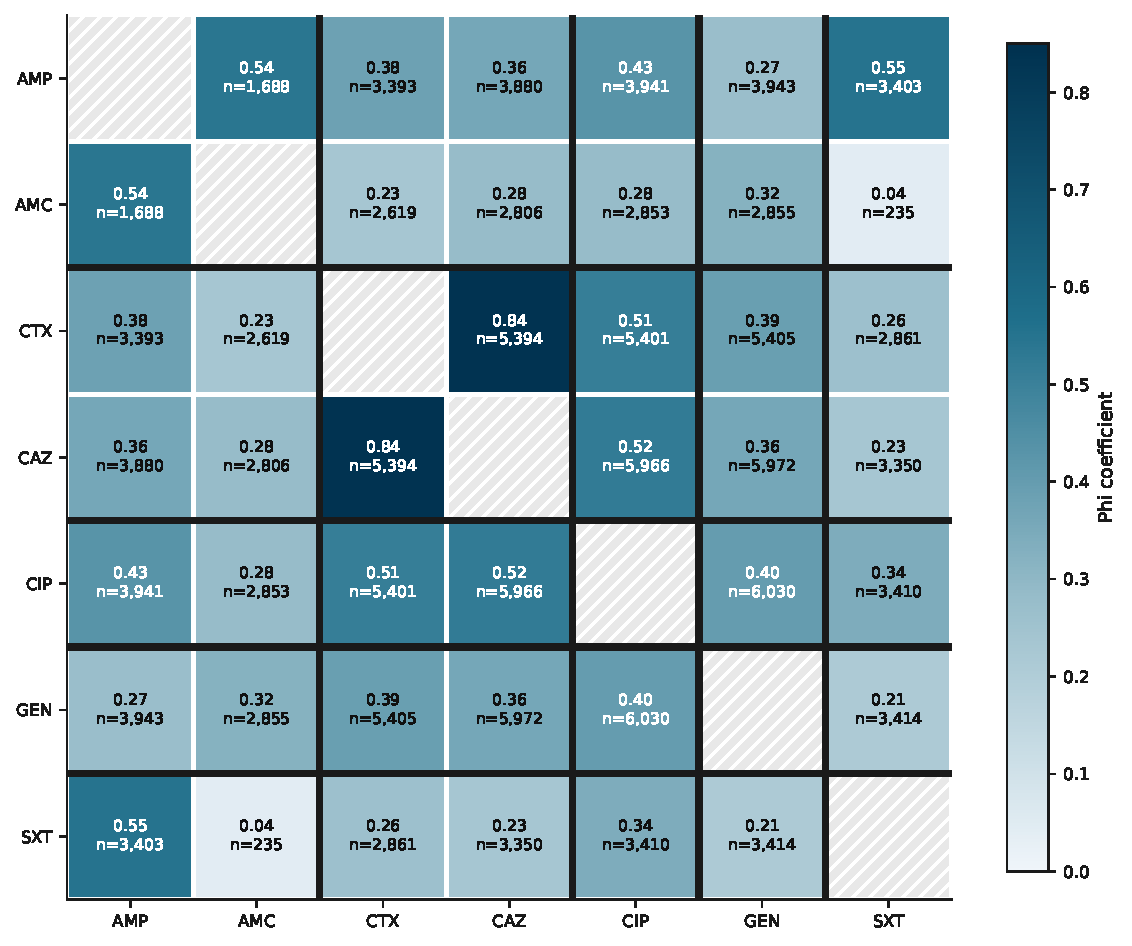
\includegraphics[width=0.62\textwidth]{fig_coresistance.pdf}
\caption{Pairwise co-resistance ($\phi$) between the seven antibiotics. Each cell is
computed only on the strains labelled for both drugs, and the number of such strains
is printed inside the cell. The lines separate drug classes. The two cephalosporins
stand out at 0.84, but below that pair the class boundaries stop predicting the
pattern.}
\label{fig:coresistance}
\end{figure*}

Of all the pairs, the two cephalosporins are by far the most similar at $\phi = 0.84$.
And that is the shared-mechanism story, precisely. However, below that, drug class
fails to predict anything useful. AMP and SXT are at 0.55 across two dissimilar
classes, greater than AMP and AMC are at 0.54 within a single class. With the two
cephalosporins, CIP, which has no partner of its own class on the panel, is at 0.51
and 0.52. The sharing of resistance genes via a plasmid or an integron causes these
to move together regardless of whether they are targeting the same drug or not,
which is demonstrated by this panel.

The figure also illustrates the reason that small values of $\phi$ cannot be ranked
in the same fashion. Some
pairs are measured on only 235 strains (AMC and SXT) while others are measured on
6{,}030 (CIP and GEN), so the numbers do not rest on the same amount of evidence.

So Lens C has a shared trunk, then five drug-class projections, and then a
co-resistance refinement step:
\begin{equation}
r = \mathrm{MLP}\big([z_C ; \ell_C^{\text{init}}]\big), \qquad
\ell_C = \ell_C^{\text{init}} + \alpha\, r
\end{equation}
Here $\alpha$ is a single learned number that starts at 0.1, so the model mostly
ignores this step at first and only leans on it when the data supports it. The step
exists because a module that shared information only inside a drug class would find
the cephalosporin link but would miss every link across classes.

\subsubsection{The Mixture-of-Experts Gate}

The three lenses now give three opinions per antibiotic, and they will not always
agree. The easy answer would be to average them, but we rejected that. Averaging
assumes all three lenses are equally useful. If resistance comes from an acquired
plasmid gene, Lens B should dominate while Lens A says almost nothing, and for a
point mutation the opposite holds. Averaging would drown the strongest opinion in
two weaker ones.

Instead the three 64-length summaries are concatenated into a 192-length vector and
passed through a small network and a softmax:
\begin{equation}
g = \mathrm{softmax}\big(\mathrm{MLP}([z_A; z_B; z_C])\big), \qquad g \in \mathbb{R}^{B \times 7 \times 3}
\end{equation}
So for every strain and every antibiotic there are three non-negative weights that
sum to one. The fused score is the weighted sum of the three lens scores.

This kind of gate has a known failure called expert collapse. Early in training one
lens is a little better by chance, so the gate gives it more weight, so it gets a
larger gradient, so it learns faster, so the gate gives it even more. After a few
epochs the other two stop learning and the model silently becomes a single-lens
network. To prevent this we measure the spread of the gate with Shannon entropy and
add a penalty to the loss:
\begin{equation}
H(g_a) = -\sum_{e=1}^{3} g_{a,e} \log g_{a,e}
\end{equation}
Entropy is highest when the three weights are equal and lowest when the gate has
collapsed. The penalty weight is 0.01, small enough to keep all three lenses alive
without forcing an even split, and we raise it automatically if any lens drops below
a threshold. With the delivered model Lens B copes with between 0.590 and 0.900 of the weight,
and we report honestly that this is a collapse that is slowed but not halted.

\subsubsection{Classical Learners and Stacking}

Alongside the neural part we train five classical models: XGBoost \cite{chen2016}
on gene features, LightGBM \cite{ke2017}, random forest \cite{breiman2001},
logistic regression, and a second XGBoost on chi-squared-filtered raw SNPs, combined
by stacked generalisation \cite{wolpert1992}.

Five may look like more than needed. An ensemble only helps when its members make
different mistakes, so we chose five that fail differently in three ways: whether a
model captures feature combinations or weighs each feature alone, how much its
answers move when training data changes slightly, and whether it reads the genome
gene by gene or variant by variant.

Each base learner is trained with five-fold cross-validation, so every strain is
predicted by a model that never saw it, and these out-of-fold predictions train the
meta-learner. This matters more than it sounds. A model scoring its own training
data looks better than it is, and the meta-learner would learn to trust those
inflated numbers. Out-of-fold prediction is what makes the stacking weights
trustworthy.

The meta-learner is an $L_2$-penalised logistic regression with $C = 1.0$, one per
antibiotic. Separate meta-learners are deliberate, because different drugs lean on
different base models and one shared meta-learner would force all seven into the
same compromise. We also tested a deeper neural meta-learner with four-head
self-attention across the drugs. It scored 0.8253 against 0.8486, so it was worse:
it stretches the meta-feature vector to 170 numbers with only about 5{,}000 training
rows behind it, so it fits noise. The linear version also has readable weights.

\subsection{Hyperparameters}

Table~\ref{tab:hyper} lists the main settings, most of which exist to control
overfitting, the main risk when 6{,}962 samples face hundreds of thousands of
candidate features. We did not run a full grid search. These are typical values that we kept constant
while we varied only what we wanted to compare.

\begin{table}[t]
\caption{Main hyperparameters.}
\label{tab:hyper}
\centering
\small
\setlength{\tabcolsep}{4pt}
\renewcommand{\arraystretch}{1.15}
\begin{tabular}{|>{\raggedright\arraybackslash}p{1.95cm}|>{\raggedright\arraybackslash}p{5.6cm}|}
\hline
\rowcolor{headgrey}
\textbf{Component} & \textbf{Settings} \\ \hline
XGBoost (gene) & n\_estimators=1500; max\_depth=5; learning\_rate=0.05; subsample=0.8; colsample\_bytree=0.7; reg\_alpha=0.1; reg\_lambda=1.0; early\_stopping\_rounds=150 \\ \hline
XGBoost (raw) & $\chi^2$ pre-filter to top 50{,}000 SNPs; n\_estimators=1500; max\_depth=5; learning\_rate=0.05; colsample\_bynode=0.5 \\ \hline
LightGBM & n\_estimators=1500; num\_leaves=63; max\_depth=6; min\_child\_samples=20; learning\_rate=0.05 \\ \hline
Random forest & n\_estimators=200; max\_depth=12; min\_samples\_leaf=10 \\ \hline
Neural lenses and gate & AdamW; learning\_rate=$10^{-3}$ with cosine annealing; weight\_decay=$10^{-4}$; batch\_size=16; up to 50 epochs; early stopping patience 8; gradient clipping at norm 1.0; entropy weight 0.01 \\ \hline
Meta-learner & Logistic regression ($L_2$, $C=1.0$), one per antibiotic, fitted on 5-fold out-of-fold inputs \\ \hline
\end{tabular}
\renewcommand{\arraystretch}{1.0}
\end{table}

The two settings require a word. The batch size is not large due to the large size
of the arrays; the SNP view alone is $6{,}962 \times 5{,}000 \times 64$. Gradient
clipping is important since attention is over 32{,}441 genes and gradients can
become large enough to disrupt training.

Class imbalance is handled by weighting. For the tree models we set
\texttt{scale\_pos\_weight} to the ratio of susceptible to resistant samples, about
7.5 for GEN. Logistic regression and random forest use balanced class weights, and
the neural lenses use positive-class weighting in the loss. We chose weighting over
synthetic oversampling because SMOTE would invent genomes no real bacterium has.

\subsection{The Three Evaluation Splits}

All three splits use the same fixed seed (42), so every number here can be
reproduced.

\textbf{Random split} (4{,}872 / 1{,}045 / 1{,}045), stratified on the AMP label.
This is what most papers report, and related strains land on both sides.

\textbf{Phylogroup-stratified split} (4{,}872 / 1{,}045 / 1{,}045), balancing the
eight-way phylogroup label across the three parts. We include it to make one point
clear: a stratified split is not a holdout. Every phylogroup appears on both sides
by design, so it never tests an unseen family. It only tests how much the result
moves when we change the balancing variable.

\textbf{Sequence-type lineage holdout} (4{,}836 / 1{,}081 / 1{,}045). This is the
real test. We found a sequence type for 6{,}487 of the 6{,}962 strains, giving 458
types, of which the largest holds 884 strains, nearly one genome in eight.

Two rules were fixed before we saw any result. A strain with no sequence type goes
to training, because a group we cannot name cannot be held out safely. And any type
larger than five per cent of the typed collection (324 strains) also goes to
training, because a test set made mostly of one clone tests nothing. Four types met
that condition, and the remaining 454 were sent whole to training, validation or
test by seeded random assignment. The part sizes are not round numbers, which is not
a mistake but evidence that whole families were kept together.

We checked the holdout twice. No sequence type appears in more than one part. And a
nearest-neighbour scan of Hamming distance from each test strain to its closest
training strain found 47 of 1{,}045 random-split test strains within 0.5\% of a
training strain, making them near-copies, against 0 of 1{,}045 under the holdout.
Removing those 47 moved the random-split score by only 0.0041 and not in one steady
direction, so near-copies do not drive our results.

\subsection{Metrics}

Our main metric is PR-AUC, because the classes are imbalanced and a precision-recall
curve is more informative than an ROC curve on imbalanced data \cite{saito2015},
while accuracy hides exactly the failure we care about. GEN shows this: categorical
agreement of 0.934 while missing 43.6\% of resistant strains.

We also report Matthews correlation, $F_1$, $F_2$, and the error terms used in
microbiology. A very major error (VME) is a resistant strain called susceptible,
which is the dangerous case. A major error (ME) is the opposite, costing a drug
option but not risking the patient. Categorical agreement (CA) is the percentage of calls that agree with the
laboratory. CLSI requests both error rates to remain less than three per cent. The
confidence intervals are based on 1{,}000 bootstrap resamples of the test set, at
2.5th and 97.5th percentiles.

\subsection{The Prevalence Correction}

Since this step in our method is novel, we provide a detailed description of it.
The one property of PR-AUC that will be important here is that its no-skill
baseline is precisely the prevalence of the positive class. A model with no skill scores the share of
resistant strains in the test set. If half are resistant, a useless model scores
0.5; if a tenth are, it scores 0.1.

Holding out the biggest families removes many resistant strains, because the big
clones happen to be the resistant ones, so the holdout test set ends up with a
smaller resistant share. Figure~\ref{fig:prev} shows the size of this shift. Under
the lineage holdout prevalence falls for \textit{every single antibiotic}, by 2.5 to
12.1 percentage points, while the random and phylogroup splits stay within 2.5
points and move both ways.

\begin{figure}[t]
\centering
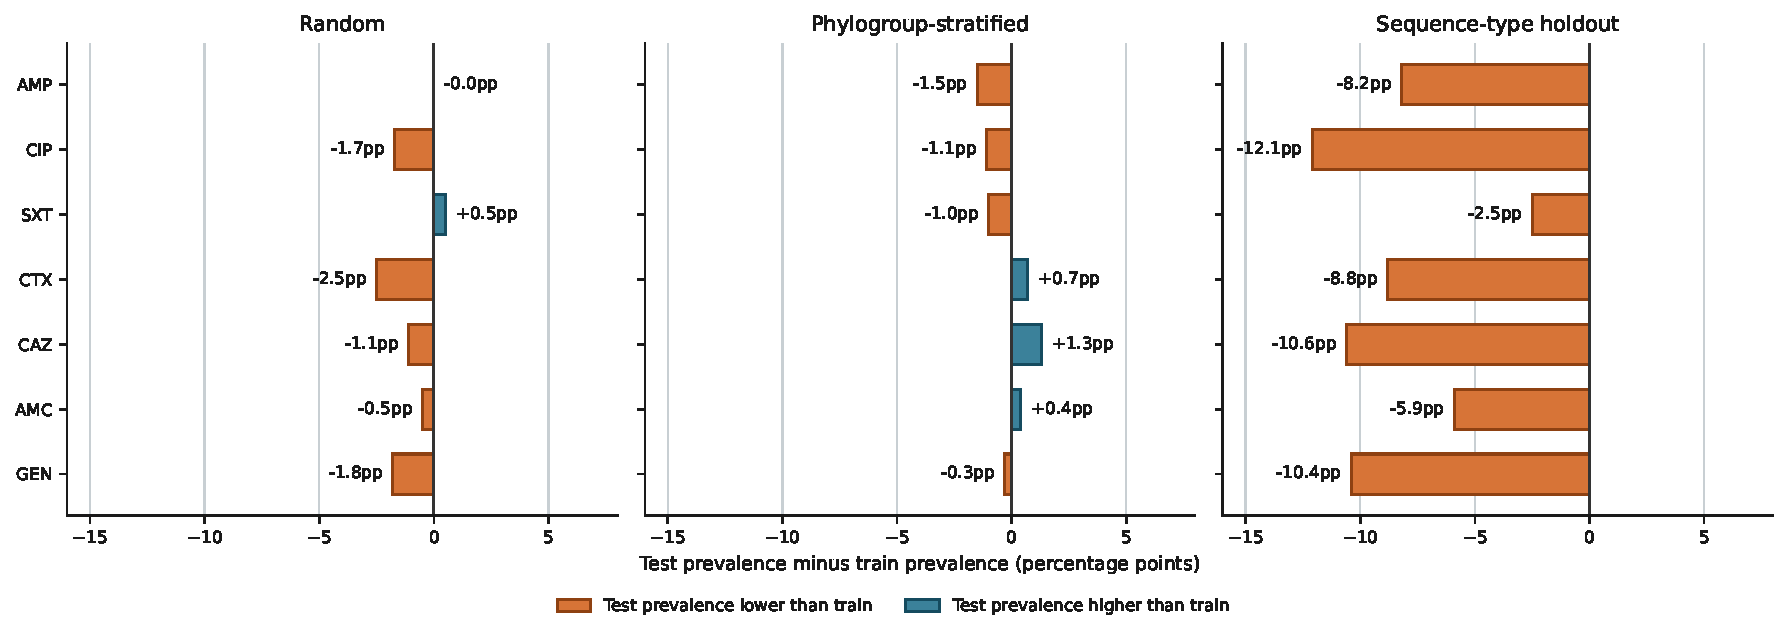
\includegraphics[width=\columnwidth]{fig_split_prevalence_shift.pdf}
\caption{Resistance prevalence in the test partition minus the training partition,
in percentage points, for each antibiotic and each split. The random and
phylogroup-stratified splits stay within 2.5 points and move both ways. The
sequence-type holdout moves downwards for every drug.}
\label{fig:prev}
\end{figure}

So PR-AUC falls even when the model ranks strains exactly as well as before. Part of
the drop is arithmetic, not model failure.

The correction works as follows. We take the saved predictions from the holdout run,
drop susceptible strains at random until the resistant share reaches a chosen target,
and recompute PR-AUC on those same saved predictions. We repeat this 2{,}000 times
and report the mean with a 95\% interval. \textbf{No model is retrained and no
resistant strain is thrown away.}

The choice of target matters, so we are exact about ours. We match to the
\textbf{training} prevalence, which answers ``how would this model score if the
holdout test set had the composition it was trained on?''

A stricter target exists and we state it rather than leave a reader to notice it.
The score we compare against, 0.8486, was measured on the random-split \textit{test}
set, whose prevalence is not identical to the training prevalence, so matching to
that test prevalence would be exactly like-for-like. We did not run it. We can bound
the difference: Fig.~\ref{fig:prev} shows the random split's test prevalence sits
within 2.5 percentage points of training for every drug, against the 2.5 to 12.1
point shift the holdout causes. The stricter target would therefore move our
corrected numbers only slightly, and in the direction of a \textit{larger} gap,
because the training prevalence is the more generous of the two. Every corrected
figure here should be read as a lower bound, which is why we say \textbf{adjusted
gap} throughout and never ``real gap''.

Because only susceptible strains are removed, the very major error rate cannot move
under this resampling at all, since it is a ratio computed inside the resistant
group. So the clinical numbers later carry no prevalence effect. We also report
ROC-AUC as an independent check, because its no-skill value is 0.5 whatever the
prevalence.

% =====================================================================
\section{Results}
\label{sec:results}
% =====================================================================

\subsection{Performance on the Random Split}

Table~\ref{tab:random} gives the full results for every antibiotic on the random
split, and Fig.~\ref{fig:prcurves} draws the matching precision-recall curves.

\begin{table}[t]
\caption{TriLens-MoE-Stack on the random split, per antibiotic. Rows are sorted by
PR-AUC.}
\label{tab:random}
\centering
\small
\setlength{\tabcolsep}{4pt}
\renewcommand{\arraystretch}{1.15}
\begin{tabular}{|l|r|r|r|r|r|}
\hline
\rowcolor{headgrey}
\textbf{Drug} & \textbf{PR-AUC} & \textbf{MCC} & \textbf{F1} & \textbf{F2} & \textbf{Acc.} \\ \hline
CIP & 0.9773 & 0.9088 & 0.9282 & 0.9197 & 0.9692 \\ \hline
AMP & 0.9440 & 0.7866 & 0.8932 & 0.8917 & 0.8933 \\ \hline
CTX & 0.9019 & 0.7904 & 0.8173 & 0.8126 & 0.9530 \\ \hline
SXT & 0.8352 & 0.6954 & 0.7875 & 0.7730 & 0.8707 \\ \hline
CAZ & 0.8299 & 0.6928 & 0.7290 & 0.7169 & 0.9356 \\ \hline
AMC & 0.7482 & 0.5237 & 0.6563 & 0.6250 & 0.8035 \\ \hline
GEN & 0.7037 & 0.6095 & 0.6386 & 0.5915 & 0.9341 \\ \hline
\rowcolor{oursblue}
\textbf{Average} & \textbf{0.8486} & \textbf{0.7153} & \textbf{0.7786} & \textbf{0.7615} & \textbf{0.9085} \\ \hline
\end{tabular}
\renewcommand{\arraystretch}{1.0}
\end{table}

\begin{figure*}[t]
\centering
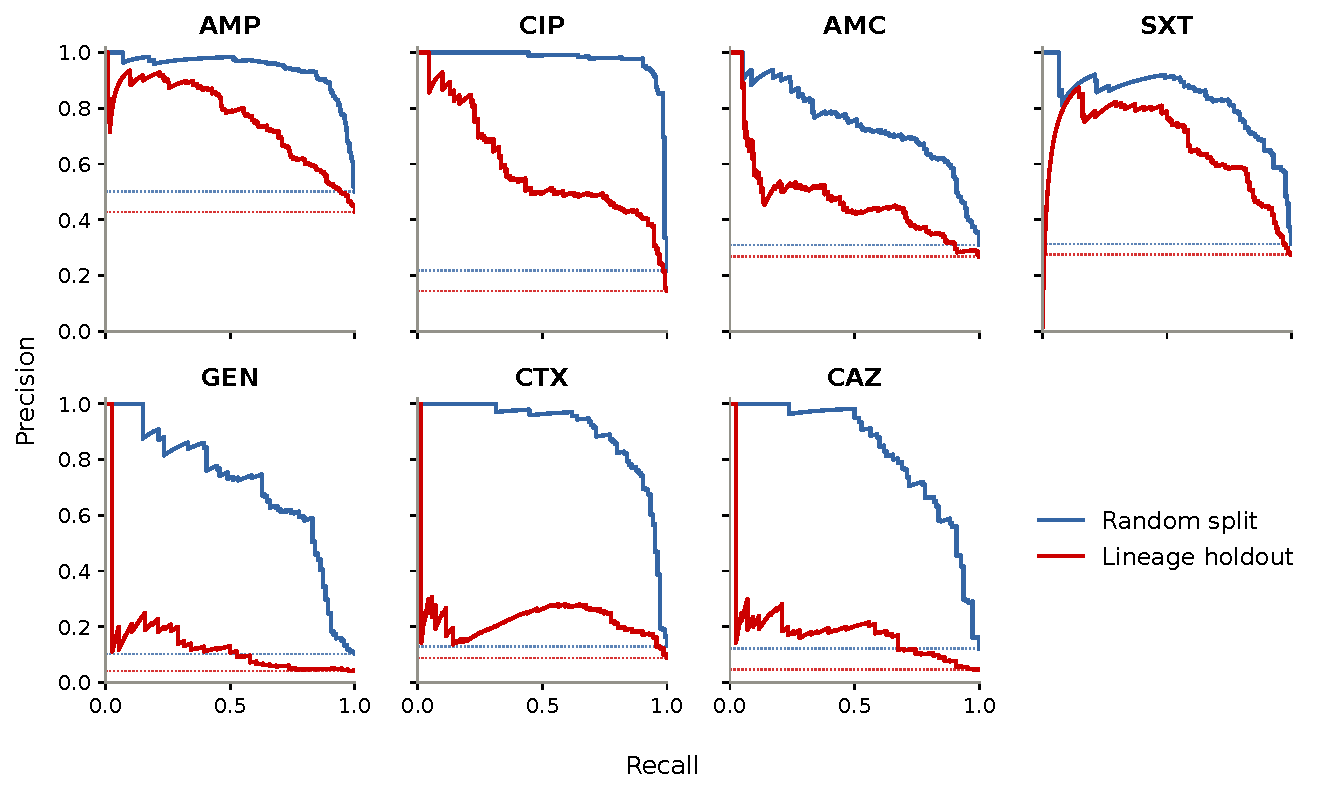
\includegraphics[width=0.94\textwidth]{fig_pr_curves.pdf}
\caption{Precision-recall curves for all seven antibiotics. Blue is the
random-split test set discussed in this subsection. Red is the sequence-type
lineage holdout, which is not analysed until later in Section~\ref{sec:results} and
is drawn here only so that the two can be compared on one set of axes. The dotted
lines are the no-skill baselines, one for each split, and they sit at the
prevalence of that split.}
\label{fig:prcurves}
\end{figure*}

The average PR-AUC is 0.8486, but that average hides a wide spread. CIP reaches
0.9773 and GEN only 0.7037, a gap of nearly 0.27 on the same genomes with the same
model. That is already a hint that the seven drugs are not one single problem.

The accuracy column behaves differently. The lowest PR-AUC but with an accuracy of
0.9341 is gained by GEN as the number of resistant strains is very small but a
model that scores high and misses the majority of the resistant cases can be
achieved. It is the pitfall we mentioned above, and the reason why accuracy is not
the primary measure.

Any comparison is measured by bootstrap intervals. CIP has the tightest,
[0.961, 0.990], because it has the most labelled data; GEN the widest,
[0.612, 0.786], a span of nearly 0.18. Before a difference between two methods is
significant, it must be larger than that width.

\subsection{How We Arrived at This Design}

Table~\ref{tab:progress} contains all the major models we constructed, in order of
building, since it justifies why the final model is a hybrid and not a pure neural
network.

\begin{table}[t]
\caption{Average PR-AUC at each stage of the project, on the curated dataset. Each
row records the score as it stood at that stage, so the gene-feature XGBoost here is
the standalone run of the time and not the base learner of the same name inside the
finished pipeline, which Table~\ref{tab:baselines} reports at 0.8375.}
\label{tab:progress}
\centering
\small
\setlength{\tabcolsep}{4pt}
\renewcommand{\arraystretch}{1.15}
\begin{tabular}{|>{\raggedright\arraybackslash}p{1.8cm}|>{\raggedright\arraybackslash}p{4.15cm}|r|}
\hline
\rowcolor{headgrey}
\textbf{Stage} & \textbf{Model} & \textbf{PR-AUC} \\ \hline
Baseline & XGBoost on 1{,}024 PCA components & 0.8033 \\ \hline
Feature engineering & XGBoost on gene-level features & 0.8297 \\ \hline
Single neural & GeneAttentionNet v1 & 0.7430 \\ \hline
Single neural & GeneAttentionNet v2 (best) & 0.7689 \\ \hline
Neural meta-stack & Deep meta-learner variant & 0.8253 \\ \hline
\rowcolor{oursblue}
\textbf{Proposed} & \textbf{TriLens-MoE-Stack} & \textbf{0.8486} \\ \hline
\end{tabular}
\renewcommand{\arraystretch}{1.0}
\end{table}

The first real improvement was obtained due to features, not model: changing from
PCA components to gene level features, the score went from 0.803 to 0.830 without
touching the learner. Our fully neural attempts disappointed. GeneAttentionNet v1 reached only
0.743, worse than a plain gradient boosting baseline, and v2 reached 0.7689 only
after seven design variants. A deeper neural meta-learner made things worse again at
0.8253. That is why we built around the classical side rather than against it, and
why we call the final model a hybrid.

\subsection{Comparison With Baselines and Components}

Table~\ref{tab:baselines} compares our model with external baselines and its own
parts.

\begin{table}[t]
\caption{External baselines and internal components, average PR-AUC across the
seven antibiotics. ``N/R'' means we did not run that configuration.}
\label{tab:baselines}
\centering
\small
\setlength{\tabcolsep}{4pt}
\renewcommand{\arraystretch}{1.15}
\begin{tabular}{|l|r|r|}
\hline
\rowcolor{headgrey}
\textbf{Model} & \textbf{Random} & \textbf{Holdout} \\ \hline
\multicolumn{3}{|l|}{\textit{External baselines}} \\ \hline
Phylogroup label only & 0.2914 & N/R \\ \hline
TabNet & 0.6951 & 0.3255 \\ \hline
XGBoost on 1{,}024 PCA components & 0.8033 & N/R \\ \hline
\multicolumn{3}{|l|}{\textit{Components of our own system}} \\ \hline
Random forest, gene features & 0.7809 & 0.4931 \\ \hline
Logistic regression, gene features & 0.7923 & 0.4408 \\ \hline
LightGBM, gene features & 0.8338 & 0.5516 \\ \hline
XGBoost, gene features & 0.8375 & 0.5507 \\ \hline
XGBoost, $\chi^2$-filtered SNPs & 0.8400 & 0.6299 \\ \hline
\rowcolor{oursblue}
\textbf{TriLens-MoE-Stack} & \textbf{0.8486} & \textbf{0.6337} \\ \hline
\end{tabular}
\renewcommand{\arraystretch}{1.0}
\end{table}

A model given only the eight-way phylogroup label, with no genome data at all,
reaches 0.2914. That is close to the average prevalence, so the broad family label
carries almost no signal alone. This rules out the simplest explanation of our
results, that the model works only because it can tell which broad family a strain
belongs to.

TabNet, a deep model built for tabular data, reaches 0.6951, behind every one of our
classical learners. Under the holdout it falls to 0.3255 while even our weakest
classical learner reaches 0.4408. So the answer here is not a deeper network.

We should also say plainly how small our own margin is. The full system beats its
own best single component by 0.0086 on the random split and 0.0038 under the
holdout. Both sit inside the bootstrap intervals, which reach about 0.18 wide for
the drug with fewest labels. That component belongs to our own system rather than a
rival method, so this is an ablation result, not a contest we won. What we defend
is the evaluation protocol and what it reveals, not the architecture.

\subsection{Component Ablation}

We also examined whether each part is justified to be there and we created three
versions with the same data, seed and test set. Stage 1 takes the average of the
three lenses and results in 0.7453. The mixture-of-experts gate is added at stage 2
and the value is 0.7807. Stage 3 introduces classical stacking and attains 0.8486.

Two things follow. Every single antibiotic improves at both steps, so no stage is
simply dead weight, although we repeat that the full stack's margin over its best
single component still sits inside the bootstrap interval. And the parts do not
help equally. The gate adds 0.0353 while classical stacking adds 0.0679, about
twice as much. So the final model is better called a hybrid than a neural model.

\subsection{What the Gate Actually Learned}

The gate adds 0.0353, so it is doing something useful. But we also checked
\textit{what} it learned, and the answer does not match our design.
Table~\ref{tab:gate} gives the average weight each lens receives per antibiotic.

\begin{table}[t]
\caption{Average gate weights on the test set. Each row sums to one.}
\label{tab:gate}
\centering
\small
\setlength{\tabcolsep}{4pt}
\renewcommand{\arraystretch}{1.15}
\begin{tabular}{|l|r|r|r|}
\hline
\rowcolor{headgrey}
\textbf{Drug} & \textbf{Lens A} & \textbf{Lens B} & \textbf{Lens C} \\ \hline
AMP & 0.070 & 0.852 & 0.078 \\ \hline
CIP & \textbf{0.035} & 0.590 & 0.374 \\ \hline
AMC & 0.095 & 0.742 & 0.163 \\ \hline
SXT & 0.052 & \textbf{0.900} & 0.047 \\ \hline
GEN & 0.098 & 0.731 & 0.171 \\ \hline
CTX & 0.064 & 0.815 & 0.121 \\ \hline
CAZ & 0.044 & 0.835 & 0.122 \\ \hline
\end{tabular}
\renewcommand{\arraystretch}{1.0}
\end{table}

Most of the weight goes to Lens B, between 0.590 and 0.900, and Lens A never rises
above 0.098. That much agrees with the biology, since a large share of resistance in
\textit{E. coli} comes from genes the bacterium picked up.

CIP is where the table stops agreeing with our design. The gate was built on a
prediction: a drug whose resistance comes from a picked-up gene should route to Lens
B, and a drug whose resistance comes from a point mutation should route to Lens A.
CIP is the clearest point-mutation drug in the panel, and it gets 0.035 on Lens A,
the lowest value in the table. The prediction fails on the one antibiotic where it
was most testable.

We should also note that four drugs sit above 0.81 on Lens B and SXT reaches 0.900.
That is close to the collapse the entropy penalty is meant to stop, so the penalty
slowed collapse down without preventing it. We therefore report the gate as a useful
way to weight the lenses, not as a way to find the resistance mechanism.

\subsection{The Lineage Holdout}

Under the sequence-type holdout the average PR-AUC falls to 0.6337, a raw drop of
0.215 from the random split.

The phylogroup-stratified split behaves very differently. It scores 0.8531, which
is \textit{higher} than the random split. Four antibiotics go up and none falls by
more than 0.022. That is not how a split that really holds back a family should
behave, and it is direct evidence that balancing and holding out answer two
different questions. We built this split first, found that it could not answer our
question, and report that as a finding.

\subsection{Applying the Prevalence Correction}

Table~\ref{tab:main} gives the per-antibiotic results across all three splits,
together with the prevalence-matched holdout and the adjusted gap.

\begin{table*}[t]
\caption{Per-antibiotic PR-AUC across the three splits, with the prevalence-matched
holdout and the resulting adjusted gap. Prevalence matching resamples the holdout
test set to the training prevalence over 2{,}000 rounds, without retraining and
without dropping any resistant strain. ROC-AUC is shown as a prevalence-independent
check. Rows are sorted by the adjusted gap, and the double line marks where the two
groups separate.}
\label{tab:main}
\centering
\small
\renewcommand{\arraystretch}{1.2}
\begin{tabular}{|l|r|r|r|l|r|r|}
\hline
\rowcolor{headgrey}
\textbf{Drug} & \textbf{Random} & \textbf{Phylogroup} & \textbf{Holdout} & \textbf{Prevalence-matched} & \textbf{ROC-AUC} & \textbf{Adjusted gap} \\ \hline
AMP & 0.9440 & 0.9338 & 0.9043 & 0.9268 \;[0.918, 0.938] & 0.9257 & $-0.017$ \\ \hline
CIP & 0.9773 & 0.9617 & 0.9118 & 0.9471 \;[0.926, 0.967] & 0.9739 & $-0.030$ \\ \hline
SXT & 0.8352 & 0.8373 & 0.7872 & 0.8046 \;[0.792, 0.823] & 0.9038 & $-0.031$ \\ \hline\hline
CTX & 0.9019 & 0.8807 & 0.6073 & 0.7260 \;[0.687, 0.766] & 0.8838 & $-0.176$ \\ \hline
CAZ & 0.8299 & 0.8481 & 0.4930 & 0.6431 \;[0.600, 0.679] & 0.7878 & $-0.187$ \\ \hline
AMC & 0.7482 & 0.7963 & 0.4865 & 0.5513 \;[0.529, 0.584] & 0.6894 & $-0.197$ \\ \hline
GEN & 0.7037 & 0.7136 & 0.2457 & 0.4594 \;[0.398, 0.511] & 0.7426 & $-0.244$ \\ \hline
\rowcolor{oursblue}
\textbf{Average} & \textbf{0.8486} & \textbf{0.8531} & \textbf{0.6337} & \textbf{0.7226} & \textbf{0.8439} & $\mathbf{-0.126}$ \\ \hline
\end{tabular}
\renewcommand{\arraystretch}{1.0}
\end{table*}

After matching, the average comes back up from 0.6337 to 0.7226. So the adjusted
gap is 0.126 and not 0.215. About two fifths of what looked like lost
generalisation was the measure and not the model.

GEN shows this most clearly. Its holdout test set keeps only 38 resistant strains,
a prevalence of 4.2 per cent against 14.6 per cent in training. Its score comes back
from 0.2457 to 0.4594, the largest recovery of the seven. Its ROC-AUC of 0.7426 had
already told us that the model was still ranking resistant strains above susceptible
ones. It had simply been asked to do so on a test set where only about one strain in
twenty-four is resistant.

AMC is the opposite case, and it shows that the correction does not just wipe our
finding away. Its prevalence changes the least, by only 5.9 points, so it comes back
the least, by 0.065 against GEN's 0.214. It also has the lowest ROC-AUC of all seven
at 0.6894. So fixing the measure does not remove the effect. It makes it clearer.

One caution applies. GEN's matched interval is wide, [0.398, 0.511], because it
rests on only 38 resistant strains, so its exact value should be read with care even
though the direction is clear. The lower-bound caveat on 0.126 stated in
Section~\ref{sec:method} applies to every row of this table.

\subsection{Our Main Finding: Two Groups of Antibiotics}

Once the measure is corrected, a pattern appears that the raw numbers hide. The last
column of Table~\ref{tab:main} shows it, and Fig.~\ref{fig:twogroups} draws it as
bars.

\begin{figure*}[t]
\centering
\resizebox{0.9\textwidth}{!}{% Random split vs lineage holdout vs prevalence-matched holdout, per antibiotic.
% Sorted by the prevalence-corrected gap, smallest first.
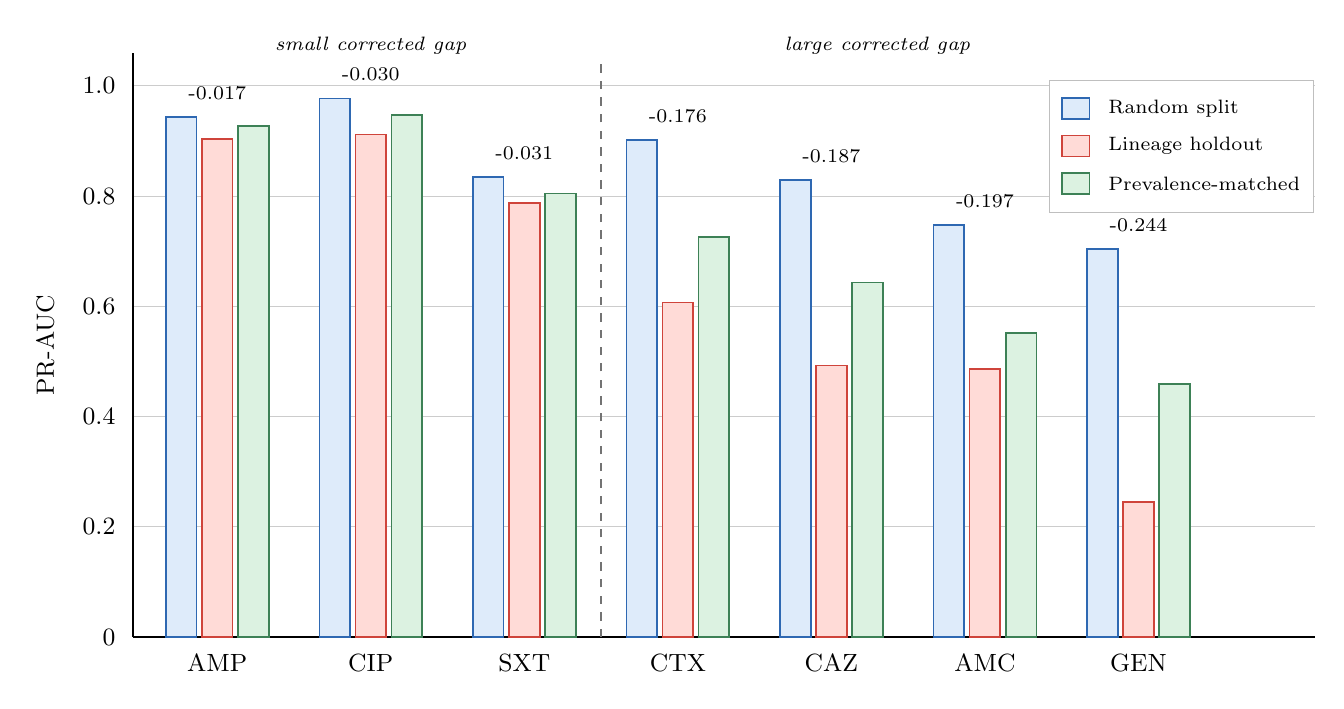
\begin{tikzpicture}[x=1.95cm, y=7.0cm]

\foreach \y in {0,0.2,0.4,0.6,0.8,1.0}{
  \draw[black!20,line width=0.4pt] (0.45,\y) -- (8.15,\y);
  \node[anchor=east,font=\small,text=black] at (0.40,\y) {\y};
}

\draw[black,line width=0.9pt] (0.45,0) -- (8.15,0);
\draw[black,line width=0.9pt] (0.45,0) -- (0.45,1.06);
\node[rotate=90,anchor=south,font=\small,text=black] at (0.00,0.53) {PR-AUC};

\foreach \i/\ab/\rnd/\hold/\mat/\gap in {%
  1/AMP/0.9440/0.9043/0.9268/{-0.017},
  2/CIP/0.9773/0.9118/0.9471/{-0.030},
  3/SXT/0.8352/0.7872/0.8046/{-0.031},
  4/CTX/0.9019/0.6073/0.7260/{-0.176},
  5/CAZ/0.8299/0.4930/0.6431/{-0.187},
  6/AMC/0.7482/0.4865/0.5513/{-0.197},
  7/GEN/0.7037/0.2457/0.4594/{-0.244}}{
    \fill[bluefill]  (\i-0.335,0) rectangle (\i-0.135,\rnd);
    \draw[blueedge,line width=0.6pt] (\i-0.335,0) rectangle (\i-0.135,\rnd);
    \fill[redfill]   (\i-0.10,0) rectangle (\i+0.10,\hold);
    \draw[rededge,line width=0.6pt] (\i-0.10,0) rectangle (\i+0.10,\hold);
    \fill[greenfill] (\i+0.135,0) rectangle (\i+0.335,\mat);
    \draw[greenedge,line width=0.6pt] (\i+0.135,0) rectangle (\i+0.335,\mat);
    \node[anchor=north,font=\small,text=black] at (\i,-0.014) {\ab};
    \node[anchor=south,font=\scriptsize,text=black] at (\i,\rnd+0.014) {\gap};
}

\draw[black!55,dashed,line width=0.8pt] (3.5,0) -- (3.5,1.04);
\node[anchor=south,font=\scriptsize\itshape,text=black,align=center]
  at (2.0,1.04) {small corrected gap};
\node[anchor=south,font=\scriptsize\itshape,text=black,align=center]
  at (5.3,1.04) {large corrected gap};

\fill[white] (6.42,0.770) rectangle (8.14,1.010);
\draw[black!25,line width=0.5pt] (6.42,0.770) rectangle (8.14,1.010);

\fill[bluefill] (6.50,0.940) rectangle (6.68,0.978);
\draw[blueedge,line width=0.6pt] (6.50,0.940) rectangle (6.68,0.978);
\node[anchor=west,font=\scriptsize,text=black] at (6.74,0.959) {Random split};

\fill[redfill] (6.50,0.872) rectangle (6.68,0.910);
\draw[rededge,line width=0.6pt] (6.50,0.872) rectangle (6.68,0.910);
\node[anchor=west,font=\scriptsize,text=black] at (6.74,0.891) {Lineage holdout};

\fill[greenfill] (6.50,0.804) rectangle (6.68,0.842);
\draw[greenedge,line width=0.6pt] (6.50,0.804) rectangle (6.68,0.842);
\node[anchor=west,font=\scriptsize,text=black] at (6.74,0.823) {Prevalence-matched};

\end{tikzpicture}
}
\caption{Random split, the lineage holdout as measured, and the same holdout after
the test set is resampled to the training prevalence. Bars are ordered by the
prevalence-corrected gap, which is printed above each group. Three antibiotics lose
0.017 to 0.031 once prevalence is corrected for, and four lose 0.176 to 0.244, with
nothing in between.}
\label{fig:twogroups}
\end{figure*}

AMP, CIP and SXT lose between 0.017 and 0.031. CTX, CAZ, AMC and GEN lose between
0.176 and 0.244. Nothing falls between 0.031 and 0.176.

This empty space is our main result. If the model had simply got worse on a harder
test, the losses would spread smoothly across all seven drugs. Instead we see two
separate groups, which suggests two different situations are being measured. In the
first group, resistance has a clear genetic marker the pan-genome captures well. CIP
is the clearest case: our analysis found \textit{gyrA} and \textit{parC}, the
textbook targets, repeating what a separate published analysis of the same
collection reported \cite{york2025}. In the second group the causing gene is not
captured well, often because it sits on a mobile element that assembles badly from
short reads, so the model leaned much more on the family label.

One piece of outside support is worth naming, because it did not come from our data.
Three of our four large-gap drugs (CTX, CAZ and AMC) are beta-lactams, and Hu et al.
\cite{hu2024}, benchmarking different tools on different collections, report that
beta-lactam F1-macro variance is exceptionally high even under random folds. Two
independent studies therefore point at the same drug class as the unstable one,
which is more than our seven points establish alone.

We remain cautious when it comes to the strength of this assertion. It is a hint,
but not a proof, that the two-group splitting occurs with the seven antibiotics. We
did not perform a formal test like the Hartigan's dip test or a permutation test of
the width of the empty band and a reviewer is correct in wanting such a test; we
note this as the first to add. Another of the tempting but erroneous readings, which
we also block: division is not chromosome versus plasmid. AMP resistance usually comes from a TEM-1 beta-lactamase on a plasmid, and
AMP sits in the small-gap group. What separates the groups is whether the causing
gene is clearly present in the assembled pan-genome, not where it physically sits.

\subsection{Clinical Error Rates}

The same division shows up in the clinical numbers, and it is even sharper there.
Table~\ref{tab:clinical} gives the error rates at a fixed threshold of 0.5, and
Fig.~\ref{fig:clinheat} shows the same numbers arranged by severity.

\begin{figure}[t]
\centering
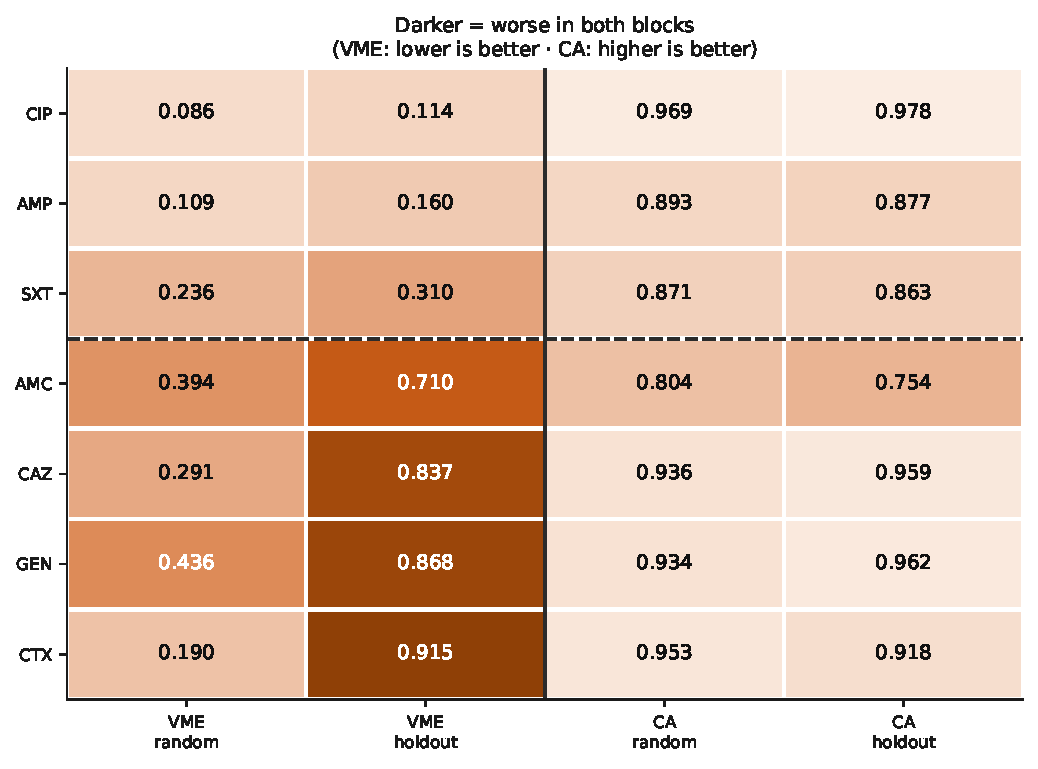
\includegraphics[width=\columnwidth]{fig_clinical_heatmap.pdf}
\caption{Very major error rate (red, lower is better) and categorical agreement
(green, higher is better), random split against lineage holdout. Drugs are ordered
by holdout VME and the dashed line marks where the two groups separate. The red
panel changes a great deal while the green panel barely moves, which is the whole
point of this subsection.}
\label{fig:clinheat}
\end{figure}

\begin{table*}[t]
\caption{Clinical error rates on the random split and under the lineage holdout, at
a fixed threshold of 0.5. Because VME and ME are both ratios computed inside one
class, neither is affected by the prevalence shift, so these numbers need no
correction. The double line marks where the two groups separate.}
\label{tab:clinical}
\centering
\small
\setlength{\tabcolsep}{5pt}
\renewcommand{\arraystretch}{1.2}
\begin{tabular}{|l|r|r|r|r|r|r|r|}
\hline
\rowcolor{headgrey}
& \textbf{Res.} & \multicolumn{3}{c|}{\cellcolor{headgrey}\textbf{VME}} & \textbf{ME} & \multicolumn{2}{c|}{\cellcolor{headgrey}\textbf{CA}} \\ \cline{3-8}
\rowcolor{headgrey}
\textbf{Drug} & \textbf{in test} & \textbf{Random} & \textbf{Holdout} & \textbf{Rise} & \textbf{Holdout} & \textbf{Random} & \textbf{Holdout} \\ \hline
CIP & 132 & 0.086 & 0.114 & $+0.028$ & 0.006 & 0.969 & 0.978 \\ \hline
AMP & 300 & 0.109 & 0.160 & $+0.051$ & 0.095 & 0.893 & 0.877 \\ \hline
SXT & 142 & 0.236 & 0.310 & $+0.074$ & 0.072 & 0.871 & 0.863 \\ \hline\hline
AMC & 145 & 0.394 & 0.710 & $+0.316$ & 0.076 & 0.804 & 0.754 \\ \hline
GEN & 38 & 0.436 & \textbf{0.868} & $+0.432$ & 0.002 & 0.934 & 0.962 \\ \hline
CAZ & 43 & 0.291 & \textbf{0.837} & $+0.546$ & 0.001 & 0.936 & 0.959 \\ \hline
CTX & 71 & 0.190 & \textbf{0.915} & $+0.725$ & 0.001 & 0.953 & 0.918 \\ \hline
\rowcolor{oursblue}
\textbf{Mean} & --- & \textbf{0.249} & \textbf{0.559} & $\mathbf{+0.310}$ & --- & --- & --- \\ \hline
\end{tabular}
\renewcommand{\arraystretch}{1.0}
\end{table*}

The mean very major error rate rises from 0.249 to 0.559. For three antibiotics the
model has more or less stopped finding resistance: it catches 6 of 71 CTX-resistant
strains, 5 of 38 GEN-resistant strains and 7 of 43 CAZ-resistant strains. In each
case the major error rate is only 0.001 or 0.002, so the model almost never says
resistant and therefore almost never raises a false alarm. That is what happens when
a classifier collapses onto the majority class.

Meanwhile categorical agreement barely moves, and for CIP, GEN and CAZ it goes
\textit{up} under the holdout. So on the metric most machine learning papers report, the model seems stable or
even improved on unseen families; on the metric a doctor cares about, it is
effectively broken. We think this contrast is the most important
practical result of our protocol.

Moving the decision threshold does not fix it. Tuning one threshold per antibiotic
on the validation set with an $F_2$ objective moved the mean VME only from 0.249 to
0.210, still far above the 0.03 limit, and forcing the major error rate inside its
limit pushed the mean VME up to 0.437. No antibiotic reached both limits at any
threshold we tried. So the problem is not where we place the cut-off but that the
model cannot separate the classes well enough. Future work belongs in the features,
not in threshold tuning.

\subsection{Which Part Survives the Holdout}

Under the lineage holdout the neural lenses alone reach 0.472 while the five
classical learners alone reach 0.628, and the full hybrid reaches 0.634. So on
strains from an unseen family the classical side does almost all the work, and
fusing the two recovers only 0.006 of the 0.156 gap between them. On the random
split the gate still adds 0.0353, so the neural part is not useless. That difference
between the two settings is itself a finding: it suggests the neural part learned
family membership more than resistance mechanism, because once families are gone
most of what it learned stops helping.

\subsection{A Problem in Gated Attention and Our Fix}

Lens B reads a vector of zeros and ones. In standard gated attention an item's score
comes from its own vector. But for a gene that is present, that vector is just the
gene's embedding, which is identical for every strain carrying the gene. So the
attention ranking came out the same for all 6{,}962 strains. Attention that should
change from sample to sample did not change at all, and could not say that one gene
matters for one particular strain, which is the whole reason for putting attention
there.

Our fix adds a context vector built from the average embedding of the genes that
strain actually carries, so every gene is scored alongside the other genes present
in the same strain:
\begin{equation}
c = \frac{1}{\max(n_b,1)}\sum_{k} \tilde{e}_k, \qquad n_b = \sum_k x_k
\end{equation}
\begin{equation}
s_k = w^{\!\top}\!\left( \tanh(V\tilde{e}_k + V_c c) \odot \sigma(U\tilde{e}_k + U_c c)\right)
\end{equation}

Table~\ref{tab:attnfix} gives the ablation. Everything else is identical between
the two columns.

\begin{table}[t]
\caption{Ablation of strain conditioning in Lens B. Only this one term changes
between the two columns.}
\label{tab:attnfix}
\centering
\small
\setlength{\tabcolsep}{4pt}
\renewcommand{\arraystretch}{1.15}
\begin{tabular}{|>{\raggedright\arraybackslash}p{3.6cm}|r|r|r|}
\hline
\rowcolor{headgrey}
\textbf{Measure} & \textbf{Standard} & \textbf{Fixed} & \textbf{Change} \\ \hline
Random split, full stack & 0.8462 & 0.8486 & $+0.0024$ \\ \hline
Phylogroup split, full stack & 0.8519 & 0.8531 & $+0.0012$ \\ \hline
Holdout, full stack & 0.6300 & 0.6337 & $+0.0037$ \\ \hline
Holdout, classical only & 0.628 & 0.628 & $\pm0$ \\ \hline
\rowcolor{oursblue}
\textbf{Holdout, neural lenses only} & \textbf{0.437} & \textbf{0.472} & $\mathbf{+0.035}$ \\ \hline\hline
Mean very major error rate & 0.257 & 0.249 & $-0.008$ \\ \hline
Resistance genes found by attention & 0 & 1 & --- \\ \hline
\end{tabular}
\renewcommand{\arraystretch}{1.0}
\end{table}

The interesting part is not the fix itself but where it shows up. The term gains
almost nothing where it is easy to measure: $+0.0024$ on the random split and
$+0.0037$ on the full stack under the holdout. It gains ten times more where it is
actually needed: $+0.035$ on the neural lenses alone under the holdout. It changes
the classical learners by exactly zero, which is what we expected, because they
never touch the attention.

An ablation run only on the random split would have hidden this completely. That is
the same argument this paper makes about testing, showing up again inside a single
term of the architecture.

\subsection{Interpretability, Reported as a Negative Result}

We extracted the most important genes from two sources: attention weights inside the
three lenses, and SHAP values \cite{lundberg2017} over the five classical learners.
This gave 1{,}138 marker genes, of which 889 (78.1\%) had a known function in the
gene function table released with the dataset. We marked the rest unknown rather
than guessing. Eight of the named markers have a known role in antibiotic
resistance: \textit{gyrA}, \textit{parC}, five multidrug efflux parts and one
beta-lactamase.

\textbf{All eight came from SHAP on the classical learners. None came from the
attention weights.} Of the 420 markers taken from the neural lenses, exactly one
matched, and only after the strain-conditioning fix above.

We ruled out two harmless explanations. Missing annotation is not the cause: all 140
markers from Lens C had a listed function and 97.9\% of those from Lens A did, yet
neither list produced a resistance gene. Too small a window is not the cause either:
repeating the check on the top 100 genes, five times our original window, raised
coverage to 79.3\% and still found none.

So what are the attended genes, if not resistance genes? We measure two ratios over
the top twenty genes per antibiotic: $U_{ST}$, the share of a gene's presence
pattern explained by its sequence type, and $U_{res}$, the share explained by the
resistance label. Table~\ref{tab:umark} compares both attribution sources against
500 random gene sets of the same size.

\begin{table}[t]
\caption{How much of each gene set is explained by lineage ($U_{ST}$) and by
resistance ($U_{res}$). The attention row is the standard formulation; the delivered
strain-conditioned lens reaches 0.357 and 0.0419.}
\label{tab:umark}
\centering
\small
\setlength{\tabcolsep}{4pt}
\renewcommand{\arraystretch}{1.15}
\begin{tabular}{|l|r|r|r|}
\hline
\rowcolor{headgrey}
\textbf{Gene set} & \textbf{$U_{ST}$} & \textbf{vs. random} & \textbf{$U_{res}$} \\ \hline
Random genes (500 draws) & 0.539 & --- & --- \\ \hline
SHAP, classical learners & 0.375 & $0.70\times$ & \textbf{0.0473} \\ \hline
Attention, Lens B & \textbf{0.312} & $0.58\times$ & \textbf{0.0192} \\ \hline
\end{tabular}
\renewcommand{\arraystretch}{1.0}
\end{table}

Two things follow. First, a random accessory gene in this pan-genome has 54\% of its
presence pattern explained by sequence type alone. That is a property of the data,
not of our model, and it is the clearest single reason a lineage-aware split was
needed. Second, the attended genes are not family markers either. At 0.312 they are
\textit{less} tied to family than a random gene, and none of the 500 random draws
fell below them. But their $U_{res}$ of 0.0192 is the lowest of the three sets,
about half what SHAP's genes carry. The classical side picks genes with two and a
half times more resistance information, which matches the fact that the classical
side is also the part that survives the holdout.

The real cause is that attention entropy sits at its maximum. Attention runs over
the 5{,}000 selected genes, so the highest possible entropy is
$\ln 5000 \approx 8.52$. The measured value reaches 8.51 for SXT and stays above
7.79 for four more drugs. The weights are almost equal, so no ranking is left to
read. The lens did not read the wrong thing; it read hardly anything.

A second disagreement on the classical side deserves reporting too. Comparing the
top twenty genes ranked by XGBoost gain with the top twenty ranked by SHAP, the
Jaccard overlap averages 0.11 on gene features and 0.17 on raw SNPs, so only four to
six genes of twenty are shared, and the rank correlation is negative for all seven
drugs. Two attribution methods on the same trained model should not disagree this
much. We therefore report the recovered genes as leads, not as an explanation of the
model. They are useful because they agree with biology other groups established
independently, not because our attribution proved them.

\subsection{External Dataset}

One collection cannot tell us whether a method works elsewhere, so we used a second,
separate set of \textit{E. coli} genomes collected at the University of Giessen and published by Ren et al. \cite{ren2022}: 809 strains with complete results for four
antibiotics, each described by 60{,}936 SNP positions. For transparency, one author
of this paper is also an author of \cite{siddiqui2025}, which uses the same Giessen
collection. The collection is public and was released by an unrelated group
\cite{ren2022}, and we use it only as an external check, never for model selection.

The two collections share no common features, because ours is built on a pan-genome
and Giessen uses one reference genome, so a model trained on our data cannot be run
on Giessen at all. Instead we rebuilt the classical stacking part of the pipeline
from scratch on Giessen with the same protocol and hyperparameters. This compares
two methods; it does not move a trained model between datasets, and we say so
clearly. The rebuilt part kept about 90\% of its score, with the drug ordering
unchanged, CIP highest and GEN lowest.

That 90\% needs a caution. Giessen's resistance prevalence is two to three times
ours for every shared drug, so the no-skill floor is higher there and the retention
percentages look better than they are, because the baseline is easier rather than
the model better. CIP shows this plainly, since its apparent retention comes out
slightly above 100\%. So we defend the weaker claim: our recipe can be rebuilt on a
separate collection and does not fall apart.

% =====================================================================
\section{Discussion}
\label{sec:discussion}
% =====================================================================

Our results support three conclusions.

\textbf{One random-split score is not enough evidence.} The same model in this paper
reports 0.849, 0.634 or 0.723 depending on how it is tested and measured, and its
very major error rate more than doubles between the first and second of those
settings while the accuracy-style measure hardly moves. Any of those three numbers
could be quoted on its own without being wrong. That is the problem.

\textbf{A lineage-aware split is needed, but it is not enough on its own.} Our
phylogroup-stratified split scored higher than the random split, which shows that
balancing families is not the same as removing one. And once a real holdout is used,
the metric itself moves, so comparing raw scores across splits mixes a real loss of
generalisation with a measurement effect. Both steps are needed. As far as we know,
the second one has not been reported before for this task.

\textbf{Generalisation depends on the antibiotic.} We think the split into two
groups is the most useful outcome for practice, because it says where a genomic
model can be trusted on an unfamiliar strain and where it cannot. One averaged score
across a drug panel hides exactly this information.

\subsection{Answers to the Research Questions}

We can now answer the five questions raised in Section~\ref{sec:intro} directly.

\textbf{RQ1, does the hybrid work:} yes, but the difference is not as big as it is
stated in the headline. It holds steady at 0.8486 and outperforms its own best
single component by 0.0086, all within the confidence interval. \textbf{RQ2, part
each part adds:} classical stacking expands 0.0679 over the 0.0353 of the gate and
under the holdout the classical learners achieve 0.628 over the 0.472 of the
lenses. \textbf{RQ3, does attention account for the model:} no. No ranking to read
because it recovered none of the eight known resistance genes SHAP have found, and
its entropy is 8.51 versus a ceiling of 8.52. \textbf{RQ4, mechanism or population
structure:} both, in varying degrees per drug which is the two-group finding.
\textbf{RQ5, is it generalisable:} to some extent. A lineage holdout is almost
completely accurate to three drugs and completely not to four, so an affirmative or
negative would be misleading.

\subsection{Limitations}

There are limits and we do not mince our words. The study is conducted on one
organism and one primary collection. That two-group separation rests on seven
antibiotics without formal statistical testing, so it is more of a clue than proof. Our interpretability
analysis takes attention arrays from the final cross-validation fold instead of the
full ensemble, which is the weakest methodological point here. We did no laboratory
validation, so the recovered genes are leads, not confirmed mechanisms. The
phylogroup assignment depends partly on a lookup table whose source we could not
confirm, although our main result rests on sequence type, which comes straight from
the strain information file. Finally, this is not a diagnostic tool: no antibiotic
met the CLSI error limits, and we report that as an unmet requirement rather than
moving the threshold until it passed.

\subsection{Future Work}

The next steps follow from those limits. Better assembly of mobile genetic elements
should help exactly the four large-gap drugs, since what they share is a causing
gene that the assembly does not represent cleanly. A holdout design guaranteeing a
minimum number of resistant strains per drug would narrow the wide intervals that
GEN's 38 resistant test strains force on us. Running the protocol on a second
species would show whether the two-group pattern is general or specific to
\textit{E. coli}. And on the model side, the honest reading of our gate and
attention results is that explaining a presence-absence vector per strain needs a
different mechanism than attention pooling, not a bigger version of the same one.

% =====================================================================
\section{Conclusion}
\label{sec:conclusion}
% =====================================================================

We tested a three-view hybrid model for genomic antibiotic resistance prediction
under a random split, a phylogroup-stratified split and a sequence-type lineage
holdout. The drop seen under the holdout is partly a side effect of PR-AUC reacting
to the prevalence change that removing families causes, and correcting for it moves
the gap from 0.215 to an adjusted 0.126. After the correction the seven antibiotics
fall into two groups with an empty space between them: three lose almost nothing and
four lose a great deal. Generalisation in this task therefore depends on each drug's
resistance mechanism.

Three further results point the same way. The gate did not route CIP to the mutation
lens, even though CIP is the clearest mutation-driven drug in the panel. Attention
recovered none of the eight known resistance genes SHAP found. And under the holdout
the neural lenses alone reach 0.472 against the classical learners' 0.628. Together
these say that most of what our neural part learned on a random split was family
membership rather than resistance biology, and that a random split is exactly the
setting where that cannot be seen.

So what we defend is a protocol, not a score. Genomic resistance prediction should
be tested with a lineage-aware split, together with the prevalence correction that
such a split makes necessary, and reported for every antibiotic instead of as one
average. Under that protocol our own model is honest about where it works: it can be
trusted on AMP, CIP and SXT for a strain from an unseen family, and not on CTX, CAZ,
AMC or GEN. No antibiotic met the CLSI error limits, so this is a research prototype
and not a clinical tool. The model produced the finding, but the way we tested it is
what made the finding visible.

\section*{Data and Code Availability}

Both genome collections used here are public. The primary collection is the Arcadia
Science \textit{E. coli} genotype and phenotype release \cite{morin2024,york2025}
and the external collection is the Giessen set of Ren et al. \cite{ren2022}. Every
split, filter and model in this paper is driven by a single fixed seed (42), and
the code, the split definitions and the saved out-of-fold predictions needed to
reproduce every number and figure will be released in a public repository on
publication.

\section*{Acknowledgment}

The authors thank the Department of Computer Science and Engineering, BRAC
University, for supporting this work.

\balance
% =====================================================================
% IEEE requires references to be numbered in the order of first citation.
% The order below matches the first \cite of each entry. Do not re-sort.
% Every entry is taken from the verified thesis bibliography (references.bib)
% and carries a full venue. Do not shorten a venue away.
\begin{thebibliography}{00}

\bibitem{murray2022} Antimicrobial Resistance Collaborators, ``Global burden of bacterial antimicrobial resistance in 2019: a systematic analysis,'' \textit{The Lancet}, vol.~399, no.~10325, pp.~629--655, 2022, doi: 10.1016/S0140-6736(21)02724-0.

\bibitem{who2025glass} World Health Organization, \textit{Global Antibiotic Resistance Surveillance Report 2025: WHO Global Antimicrobial Resistance and Use Surveillance System (GLASS)}. Geneva, Switzerland: WHO, 2025, ISBN 978-92-4-011633-7.

\bibitem{naghavi2024} M. Naghavi \textit{et al.}, ``Global burden of bacterial antimicrobial resistance 1990--2021: a systematic analysis with forecasts to 2050,'' \textit{The Lancet}, vol.~404, no.~10459, pp.~1199--1226, 2024, doi: 10.1016/S0140-6736(24)01867-1.

\bibitem{ren2022} Y. Ren, T. Chakraborty, S. Doijad, L. Falgenhauer, J. Falgenhauer, A. Goesmann, A.-C. Hauschild, O. Schwengers, and D. Heider, ``Prediction of antimicrobial resistance based on whole-genome sequencing and machine learning,'' \textit{Bioinformatics}, vol.~38, no.~2, pp.~325--334, 2022, doi: 10.1093/bioinformatics/btab681.

\bibitem{who2019} World Health Organization, \textit{No Time to Wait: Securing the Future from Drug-Resistant Infections}. Geneva, Switzerland: WHO, 2019.

\bibitem{moradigaravand2018} D. Moradigaravand, M. Palm, A. Farewell, V. Mustonen, J. Warringer, and L. Parts, ``Prediction of antibiotic resistance in \textit{Escherichia coli} from large-scale pan-genome data,'' \textit{PLOS Computational Biology}, vol.~14, no.~12, p.~e1006258, 2018, doi: 10.1371/journal.pcbi.1006258.

\bibitem{wang2025} Y. Wang, S. Zheng, R. Guo, Y. Li, H. Yin, X. Qiu, J. Chen, C. Ni, Y. Yuan, and Y. Gong, ``Assessment for antibiotic resistance in \textit{Helicobacter pylori}: a practical and interpretable machine learning model based on genome-wide genetic variation,'' \textit{Virulence}, vol.~16, no.~1, p.~2481503, 2025, doi: 10.1080/21505594.2025.2481503.

\bibitem{yu2025} Y. Yu, N. E. Wheeler, and L. Barquist, ``Biased sampling driven by bacterial population structure confounds machine learning prediction of antimicrobial resistance,'' \textit{PLOS Biology}, vol.~23, no.~12, p.~e3003539, 2025, doi: 10.1371/journal.pbio.3003539.

\bibitem{hu2024} K. Hu, F. Meyer, Z.-L. Deng, E. Asgari, T.-H. Kuo, P. C. M\"{u}nch, and A. C. McHardy, ``Assessing computational predictions of antimicrobial resistance phenotypes from microbial genomes,'' \textit{Briefings in Bioinformatics}, vol.~25, no.~3, p.~bbae206, 2024, doi: 10.1093/bib/bbae206.

\bibitem{her2018} H.-L. Her and Y.-W. Wu, ``A pan-genome-based machine learning approach for predicting antimicrobial resistance activities of the \textit{Escherichia coli} strains,'' \textit{Bioinformatics}, vol.~34, no.~13, pp.~i89--i95, 2018, doi: 10.1093/bioinformatics/bty276.

\bibitem{serajian2024} M. Serajian, S. Marini, J. N. Alanko, N. R. Noyes, M. Prosperi, and C. Boucher, ``Scalable de novo classification of antibiotic resistance of \textit{Mycobacterium tuberculosis},'' \textit{Bioinformatics}, vol.~40, no.~Suppl.~1, pp.~i39--i47, 2024, doi: 10.1093/bioinformatics/btae243.

\bibitem{gao2024} Y. Gao, H. Li, C. Zhao, S. Li, G. Yin, and H. Wang, ``Machine learning and feature extraction for rapid antimicrobial resistance prediction of \textit{Acinetobacter baumannii} from whole-genome sequencing data,'' \textit{Frontiers in Microbiology}, vol.~14, p.~1320312, 2024, doi: 10.3389/fmicb.2023.1320312.

\bibitem{do2024} D. T. Do, M.-R. Yang, T. N. S. Vo, N. Q. K. Le, and Y.-W. Wu, ``Unitig-centered pan-genome machine learning approach for predicting antibiotic resistance and discovering novel resistance genes in bacterial strains,'' \textit{Computational and Structural Biotechnology Journal}, vol.~23, pp.~1864--1876, 2024, doi: 10.1016/j.csbj.2024.04.035.

\bibitem{siddiqui2025} M. S. B. Siddiqui and N. Tarannum, ``Fusing sequence motifs and pan-genomic features: antimicrobial resistance prediction using an explainable lightweight 1D CNN--XGBoost ensemble,'' in \textit{Proc. Supercomputing Asia and Int. Conf. High Performance Computing in Asia-Pacific Region (SCA/HPCAsia)}, 2026, doi: 10.1145/3773656.3773682.

\bibitem{grinsztajn2022} L. Grinsztajn, E. Oyallon, and G. Varoquaux, ``Why do tree-based models still outperform deep learning on typical tabular data?,'' in \textit{Advances in Neural Information Processing Systems 35 (NeurIPS), Datasets and Benchmarks Track}, 2022, pp.~507--520.

\bibitem{shwartzziv2022} R. Shwartz-Ziv and A. Armon, ``Tabular data: deep learning is not all you need,'' \textit{Information Fusion}, vol.~81, pp.~84--90, 2022, doi: 10.1016/j.inffus.2021.11.011.

\bibitem{arik2021} S. \"{O}. Arik and T. Pfister, ``TabNet: attentive interpretable tabular learning,'' in \textit{Proc. AAAI Conf. Artificial Intelligence}, vol.~35, no.~8, 2021, pp.~6679--6687.

\bibitem{wolpert1992} D. H. Wolpert, ``Stacked generalization,'' \textit{Neural Networks}, vol.~5, no.~2, pp.~241--259, 1992, doi: 10.1016/S0893-6080(05)80023-1.

\bibitem{nsubuga2024} M. Nsubuga, R. Galiwango, D. Jjingo, and G. Mboowa, ``Generalizability of machine learning in predicting antimicrobial resistance in \textit{E. coli}: a multi-country case study in Africa,'' \textit{BMC Genomics}, vol.~25, p.~287, 2024, doi: 10.1186/s12864-024-10214-4.

\bibitem{saber2020} M. M. Saber and B. J. Shapiro, ``Benchmarking bacterial genome-wide association study methods using simulated genomes and phenotypes,'' \textit{Microbial Genomics}, vol.~6, no.~3, p.~e000337, 2020, doi: 10.1099/mgen.0.000337.

\bibitem{lees2020} J. A. Lees, T. T. Mai, M. Galardini, N. E. Wheeler, S. T. Horsfield, J. Parkhill, and J. Corander, ``Improved prediction of bacterial genotype-phenotype associations using interpretable pangenome-spanning regressions,'' \textit{mBio}, vol.~11, no.~4, p.~e01344-20, 2020, doi: 10.1128/mBio.01344-20.

\bibitem{yun2024} B. Yun, X. Liao, J. Feng, and T. Ding, ``Machine learning-enabled prediction of antimicrobial resistance in foodborne pathogens,'' \textit{CyTA -- Journal of Food}, vol.~22, no.~1, pp.~1--12, 2024, doi: 10.1080/19476337.2024.2324024.

\bibitem{arangoargoty2018} G. Arango-Argoty, E. Garner, A. Pruden, L. S. Heath, P. Vikesland, and L. Zhang, ``DeepARG: a deep learning approach for predicting antibiotic resistance genes from metagenomic data,'' \textit{Microbiome}, vol.~6, p.~23, 2018, doi: 10.1186/s40168-018-0401-z.

\bibitem{orcales2024} F. Orcales, L. Moctezuma Tan, M. Johnson-Hagler, J. M. Suntay, J. Ali, K. Recto, P. Glenn, and P. Pennings, ``Using genomic data and machine learning to predict antibiotic resistance: a tutorial paper,'' \textit{PLOS Computational Biology}, vol.~20, no.~12, p.~e1012579, 2024, doi: 10.1371/journal.pcbi.1012579.

\bibitem{morin2024} M. Morin, ``Creating a 7,000-strain \textit{E. coli} genotype dataset with antimicrobial resistance phenotypes,'' \textit{The Stacks}, Arcadia Science, 2024, doi: 10.57844/arcadia-d2cf-ebe5.

\bibitem{york2025} R. York and G. Sandler, ``Predicting antimicrobial resistance phenotypes across 7,000 \textit{E. coli} genomes,'' \textit{The Stacks}, Arcadia Science, 2025, doi: 10.57844/arcadia-8391-465f.

\bibitem{ilse2018} M. Ilse, J. M. Tomczak, and M. Welling, ``Attention-based deep multiple instance learning,'' in \textit{Proc. 35th Int. Conf. Machine Learning (ICML)}, 2018, pp.~2127--2136.

\bibitem{chen2016} T. Chen and C. Guestrin, ``XGBoost: a scalable tree boosting system,'' in \textit{Proc. 22nd ACM SIGKDD Int. Conf. Knowledge Discovery and Data Mining}, 2016, pp.~785--794, doi: 10.1145/2939672.2939785.

\bibitem{ke2017} G. Ke, Q. Meng, T. Finley, T. Wang, W. Chen, W. Ma, Q. Ye, and T.-Y. Liu, ``LightGBM: a highly efficient gradient boosting decision tree,'' in \textit{Advances in Neural Information Processing Systems 30 (NeurIPS)}, 2017, pp.~3146--3154.

\bibitem{breiman2001} L. Breiman, ``Random forests,'' \textit{Machine Learning}, vol.~45, no.~1, pp.~5--32, 2001, doi: 10.1023/A:1010933404324.

\bibitem{saito2015} T. Saito and M. Rehmsmeier, ``The precision-recall plot is more informative than the ROC plot when evaluating binary classifiers on imbalanced datasets,'' \textit{PLOS ONE}, vol.~10, no.~3, p.~e0118432, 2015, doi: 10.1371/journal.pone.0118432.

\bibitem{lundberg2017} S. M. Lundberg and S.-I. Lee, ``A unified approach to interpreting model predictions,'' in \textit{Advances in Neural Information Processing Systems 30 (NeurIPS)}, 2017, pp.~4765--4774.

\end{thebibliography}

\end{document}
